%%%%%%%%%%%%%%%%%%%%%%%%%%%%%%%%%%%%%%%%%
% Classicthesis Typographic Thesis
% LaTeX Template
% Version 1.3 (15/2/14)
%
% This template has been downloaded from:
% http://www.LaTeXTemplates.com
%
% Original author:
% André Miede (http://www.miede.de)
%
% License:
% CC BY-NC-SA 3.0 (http://creativecommons.org/licenses/by-nc-sa/3.0/)
%
% General Tips:
% 1) Make sure to edit the classicthesis-config.file
% 2) New enumeration (A., B., C., etc in small caps): \begin{aenumerate} \end{aenumerate}
% 3) For margin notes: \marginpar or \graffito{}
% 4) Do not use bold fonts in this style, it is designed around them
% 5) Use tables as in the examples
% 6) See classicthesis-preamble.sty for useful commands
%
%%%%%%%%%%%%%%%%%%%%%%%%%%%%%%%%%%%%%%%%%

%----------------------------------------------------------------------------------------
%	PACKAGES AND OTHER DOCUMENT CONFIGURATIONS
%----------------------------------------------------------------------------------------

\documentclass[titlepage,numbers=noenddot,headinclude,footinclude=true,cleardoublepage=empty,paper=a4,fontsize=11pt,american]{scrreprt} 
                
% Includes the file which contains all the document configurations and packages - make sure to edit this file
%%%%%%%%%%%%%%%%%%%%%%%%%%%%%%%%%%%%%%%%%
% Thesis Configuration File
%
% The main lines to change in this file are in the DOCUMENT VARIABLES
% section, the rest of the file is for advanced configuration.
%
%%%%%%%%%%%%%%%%%%%%%%%%%%%%%%%%%%%%%%%%%

%----------------------------------------------------------------------------------------
%	DOCUMENT VARIABLES
%	Fill in the lines below to enter your information into the thesis template
%	Each of the commands can be cited anywhere in the thesis
%----------------------------------------------------------------------------------------

% Remove drafting to get rid of the '[ Date - classicthesis version 4.0 ]' text at the bottom of every page
\PassOptionsToPackage{eulerchapternumbers,listings, pdfspacing, subfig,beramono,parts}{classicthesis}
% Available options: drafting parts nochapters linedheaders eulerchapternumbers beramono eulermath pdfspacing minionprospacing tocaligned dottedtoc manychapters listings floatperchapter subfig
% Adding 'dottedtoc' will make page numbers in the table of contents flushed right with dots leading to them

\newcommand{\myTitle}{Numerical Simulation of One Way Quantum Computation with Error Correction \xspace}
\newcommand{\mySubtitle}{MSc Project Report\xspace}
\newcommand{\myDegree}{MSc Quantum Technologies\xspace}
\newcommand{\myName}{John Children\xspace}
\newcommand{\myProf}{Tim Spiller\xspace}
\newcommand{\myOtherProf}{Put name here\xspace}
\newcommand{\mySupervisor}{Jaewoo Joo\xspace}
\newcommand{\myFaculty}{Put data here\xspace}
\newcommand{\myDepartment}{Physics and Astronomy\xspace}
\newcommand{\myUni}{University of Leeds\xspace}
\newcommand{\myLocation}{Leeds\xspace}
\newcommand{\myTime}{September 2014\xspace}
\newcommand{\myVersion}{version 1.2\xspace}

%----------------------------------------------------------------------------------------
%	USEFUL COMMANDS
%----------------------------------------------------------------------------------------

\newcommand{\ie}{i.\,e.}
\newcommand{\Ie}{I.\,e.}
\newcommand{\eg}{e.\,g.}
\newcommand{\Eg}{E.\,g.} 

\newcounter{dummy} % Necessary for correct hyperlinks (to index, bib, etc.)
\providecommand{\mLyX}{L\kern-.1667em\lower.25em\hbox{Y}\kern-.125emX\@}

%----------------------------------------------------------------------------------------
%	PACKAGES
%----------------------------------------------------------------------------------------

\usepackage{lipsum} % Used for inserting dummy 'Lorem ipsum' text into the template

%------------------------------------------------
 
\PassOptionsToPackage{latin9}{inputenc} % latin9 (ISO-8859-9) = latin1+"Euro sign"
\usepackage{inputenc}
 
 %------------------------------------------------

%\PassOptionsToPackage{ngerman,american}{babel}  % Change this to your language(s)
% Spanish languages need extra options in order to work with this template
%\PassOptionsToPackage{spanish,es-lcroman}{babel}
\usepackage{babel}

%------------------------------------------------			

\PassOptionsToPackage{square,numbers}{natbib}
 \usepackage{natbib}
 
 %------------------------------------------------

\PassOptionsToPackage{fleqn}{amsmath} % Math environments and more by the AMS 
 \usepackage{amsmath}
 
 %------------------------------------------------

\PassOptionsToPackage{T1}{fontenc} % T2A for cyrillics
\usepackage{fontenc}

%------------------------------------------------

\usepackage{xspace} % To get the spacing after macros right

%------------------------------------------------

%\usepackage{pdfpages} % pdf pages in document

%------------------------------------------------

\usepackage{mparhack} % To get marginpar right

%------------------------------------------------

\usepackage{scrhack} % To remove float errors on compile


%------------------------------------------------

\usepackage{fixltx2e} % Fixes some LaTeX stuff 

%------------------------------------------------

\usepackage{braket} % Enables braket notation

%------------------------------------------------

\PassOptionsToPackage{smaller}{acronym} % Include printonlyused in the first bracket to only show acronyms used in the text
\usepackage{acronym} % nice macros for handling all acronyms in the thesis

%------------------------------------------------

%\renewcommand*{\acsfont}[1]{\textssc{#1}} % For MinionPro
\renewcommand{\bflabel}[1]{{#1}\hfill} % Fix the list of acronyms

%------------------------------------------------

\PassOptionsToPackage{pdftex}{graphicx}
\usepackage{graphicx} 

%----------------------------------------------------------------------------------------
%	FLOATS: TABLES, FIGURES AND CAPTIONS SETUP
%----------------------------------------------------------------------------------------

\usepackage{tabularx} % Better tables
\setlength{\extrarowheight}{3pt} % Increase table row height
\newcommand{\tableheadline}[1]{\multicolumn{1}{c}{\spacedlowsmallcaps{#1}}}
\newcommand{\myfloatalign}{\centering} % To be used with each float for alignment
\usepackage{caption}
\captionsetup{format=hang,font=small}
\usepackage{subfig}  

%----------------------------------------------------------------------------------------
%	CODE LISTINGS SETUP
%----------------------------------------------------------------------------------------

\usepackage{listings} 
%\lstset{emph={trueIndex,root},emphstyle=\color{BlueViolet}}%\underbar} % for special keywords
\lstset{language=Fortran, % Specify the language for listings here
keywordstyle=\color{RoyalBlue}, % Add \bfseries for bold
basicstyle=\small\ttfamily, % Makes listings a smaller font size and a different font
%identifierstyle=\color{NavyBlue}, % Color of text inside brackets
commentstyle=\color{Green}\ttfamily, % Color of comments
stringstyle=\rmfamily, % Font type to use for strings
numbers=none, % Change left to none to remove line numbers
%numberstyle=\scriptsize, % Font size of the line numbers
%stepnumber=5, % Increment of line numbers
%numbersep=8pt, % Distance of line numbers from code listing
showstringspaces=false, % Sets whether spaces in strings should appear underlined
breaklines=true, % Force the code to stay in the confines of the listing box
%frameround=ftff, % Uncomment for rounded frame
frame=none, % Frame border - none/leftline/topline/bottomline/lines/single/shadowbox/L
belowcaptionskip=.75\baselineskip % Space after the "Listing #: Desciption" text and the listing box
}

\newcommand{\insertcode}[2]{\begin{itemize}\item[]\lstinputlisting[caption=#2,label=#1]{#1}\end{itemize}} % The first argument is the script location/filename and the second is a caption for the listing

%----------------------------------------------------------------------------------------
%	HYPERREFERENCES
%----------------------------------------------------------------------------------------

\PassOptionsToPackage{pdftex,hyperfootnotes=false,pdfpagelabels}{hyperref}
\usepackage{hyperref}  % backref linktocpage pagebackref
\pdfcompresslevel=9
\pdfadjustspacing=1

\hypersetup{
% Uncomment the line below to remove all links (to references, figures, tables, etc)
%draft, 
colorlinks=true, linktocpage=true, pdfstartpage=3, pdfstartview=FitV,
% Uncomment the line below if you want to have black links (e.g. for printing black and white)
%colorlinks=false, linktocpage=false, pdfborder={0 0 0}, pdfstartpage=3, pdfstartview=FitV, 
breaklinks=true, pdfpagemode=UseNone, pageanchor=true, pdfpagemode=UseOutlines,
plainpages=false, bookmarksnumbered, bookmarksopen=true, bookmarksopenlevel=1,
hypertexnames=true, pdfhighlight=/O, urlcolor=webbrown, linkcolor=RoyalBlue, citecolor=webgreen,
%------------------------------------------------
% PDF file meta-information
pdftitle={\myTitle},
pdfauthor={\textcopyright\ \myName, \myUni, \myFaculty},
pdfsubject={},
pdfkeywords={},
pdfcreator={pdfLaTeX},
pdfproducer={LaTeX with hyperref and classicthesis}
%------------------------------------------------
}   

%----------------------------------------------------------------------------------------
%	BACKREFERENCES
%----------------------------------------------------------------------------------------

\usepackage{ifthen} % Allows the user of the \ifthenelse command
\newboolean{enable-backrefs} % Variable to enable backrefs in the bibliography
\setboolean{enable-backrefs}{false} % Variable value: true or false

\newcommand{\backrefnotcitedstring}{\relax} % (Not cited.)
\newcommand{\backrefcitedsinglestring}[1]{(Cited on page~#1.)}
\newcommand{\backrefcitedmultistring}[1]{(Cited on pages~#1.)}
\ifthenelse{\boolean{enable-backrefs}} % If backrefs were enabled
{
\PassOptionsToPackage{hyperpageref}{backref}
\usepackage{backref} % to be loaded after hyperref package 
\renewcommand{\backreftwosep}{ and~} % separate 2 pages
\renewcommand{\backreflastsep}{, and~} % separate last of longer list
\renewcommand*{\backref}[1]{}  % disable standard
\renewcommand*{\backrefalt}[4]{% detailed backref
\ifcase #1 
\backrefnotcitedstring
\or
\backrefcitedsinglestring{#2}
\else
\backrefcitedmultistring{#2}
\fi}
}{\relax} 

%----------------------------------------------------------------------------------------
%	AUTOREFERENCES SETUP
%	Redefines how references in text are prefaced for different 
%	languages (e.g. "Section 1.2" or "section 1.2")
%----------------------------------------------------------------------------------------

\makeatletter
\@ifpackageloaded{babel}
{
\addto\extrasamerican{
\renewcommand*{\figureautorefname}{Figure}
\renewcommand*{\tableautorefname}{Table}
\renewcommand*{\partautorefname}{Part}
\renewcommand*{\chapterautorefname}{Chapter}
\renewcommand*{\sectionautorefname}{Section}
\renewcommand*{\subsectionautorefname}{Section}
\renewcommand*{\subsubsectionautorefname}{Section}
}
\addto\extrasngerman{
\renewcommand*{\paragraphautorefname}{Absatz}
\renewcommand*{\subparagraphautorefname}{Unterabsatz}
\renewcommand*{\footnoteautorefname}{Fu\"snote}
\renewcommand*{\FancyVerbLineautorefname}{Zeile}
\renewcommand*{\theoremautorefname}{Theorem}
\renewcommand*{\appendixautorefname}{Anhang}
\renewcommand*{\equationautorefname}{Gleichung}
\renewcommand*{\itemautorefname}{Punkt}
}
\providecommand{\subfigureautorefname}{\figureautorefname} % Fix to getting autorefs for subfigures right
}{\relax}
\makeatother

%----------------------------------------------------------------------------------------

\usepackage{classicthesis} 

%----------------------------------------------------------------------------------------
%	CHANGING TEXT AREA 
%----------------------------------------------------------------------------------------

%\linespread{1.05} % a bit more for Palatino
%\areaset[current]{312pt}{761pt} % 686 (factor 2.2) + 33 head + 42 head \the\footskip
%\setlength{\marginparwidth}{7em}%
%\setlength{\marginparsep}{2em}%

%----------------------------------------------------------------------------------------
%	USING DIFFERENT FONTS
%----------------------------------------------------------------------------------------

%\usepackage[oldstylenums]{kpfonts} % oldstyle notextcomp
%\usepackage[osf]{libertine}
%\usepackage{hfoldsty} % Computer Modern with osf
%\usepackage[light,condensed,math]{iwona}
%\renewcommand{\sfdefault}{iwona}
%\usepackage{lmodern} % <-- no osf support :-(
%\usepackage[urw-garamond]{mathdesign} <-- no osf support :-(

\begin{document}

\frenchspacing % Reduces space after periods to make text more compact

\raggedbottom % Makes all pages the height of the text on that page

\selectlanguage{american} % Select your default language - e.g. american or ngerman

%\renewcommand*{\bibname}{new name} % Uncomment to change the name of the bibliography
%\setbibpreamble{} % Uncomment to include a preamble to the bibliography - some text before the reference list starts

\pagenumbering{roman} % Roman page numbering prior to the start of the thesis content (i, ii, iii, etc)

\pagestyle{plain} % Suppress headers for the pre-content pages

%----------------------------------------------------------------------------------------
%	PRE-CONTENT THESIS PAGES
%----------------------------------------------------------------------------------------

% Title Page

\begin{titlepage}

\begin{addmargin}[-1cm]{-3cm}
\begin{center}
\large

\hfill
\vfill

\begingroup
\color{Maroon}\spacedallcaps{\myTitle} \\ \bigskip % Thesis title
\endgroup

\spacedlowsmallcaps{\myName} % Your name

\vfill


\includegraphics[width=12cm]{gfx/leedslogo} \\ \medskip % Picture

\mySubtitle \\ \medskip % Thesis subtitle
\myDegree \\
\myDepartment \\
%\myFaculty \\
\myUni \\ \bigskip

\myTime\ -- \myVersion % Time and version

\vfill

\end{center}
\end{addmargin}

\end{titlepage} % Main title page

%% Back of the title page

\thispagestyle{empty}

\hfill

\vfill

\noindent\myName: \textit{\myTitle,} \mySubtitle, %\myDegree, 
\textcopyright\ \myTime

% You may wish to do something with the back of the title page, such as including your supervisors, location or time frame of the work. Below is an example of doing so although you may want to tweak it to your liking.

%\bigskip

%\noindent\spacedlowsmallcaps{Supervisors}: \\
%\myProf \\
%\myOtherProf \\ 
%\mySupervisor

%\medskip \\

%\noindent\spacedlowsmallcaps{Location}: \\
%\myLocation

%\medskip \\

%\noindent\spacedlowsmallcaps{Time Frame}: \\
%\myTime
 % Back of the title page

%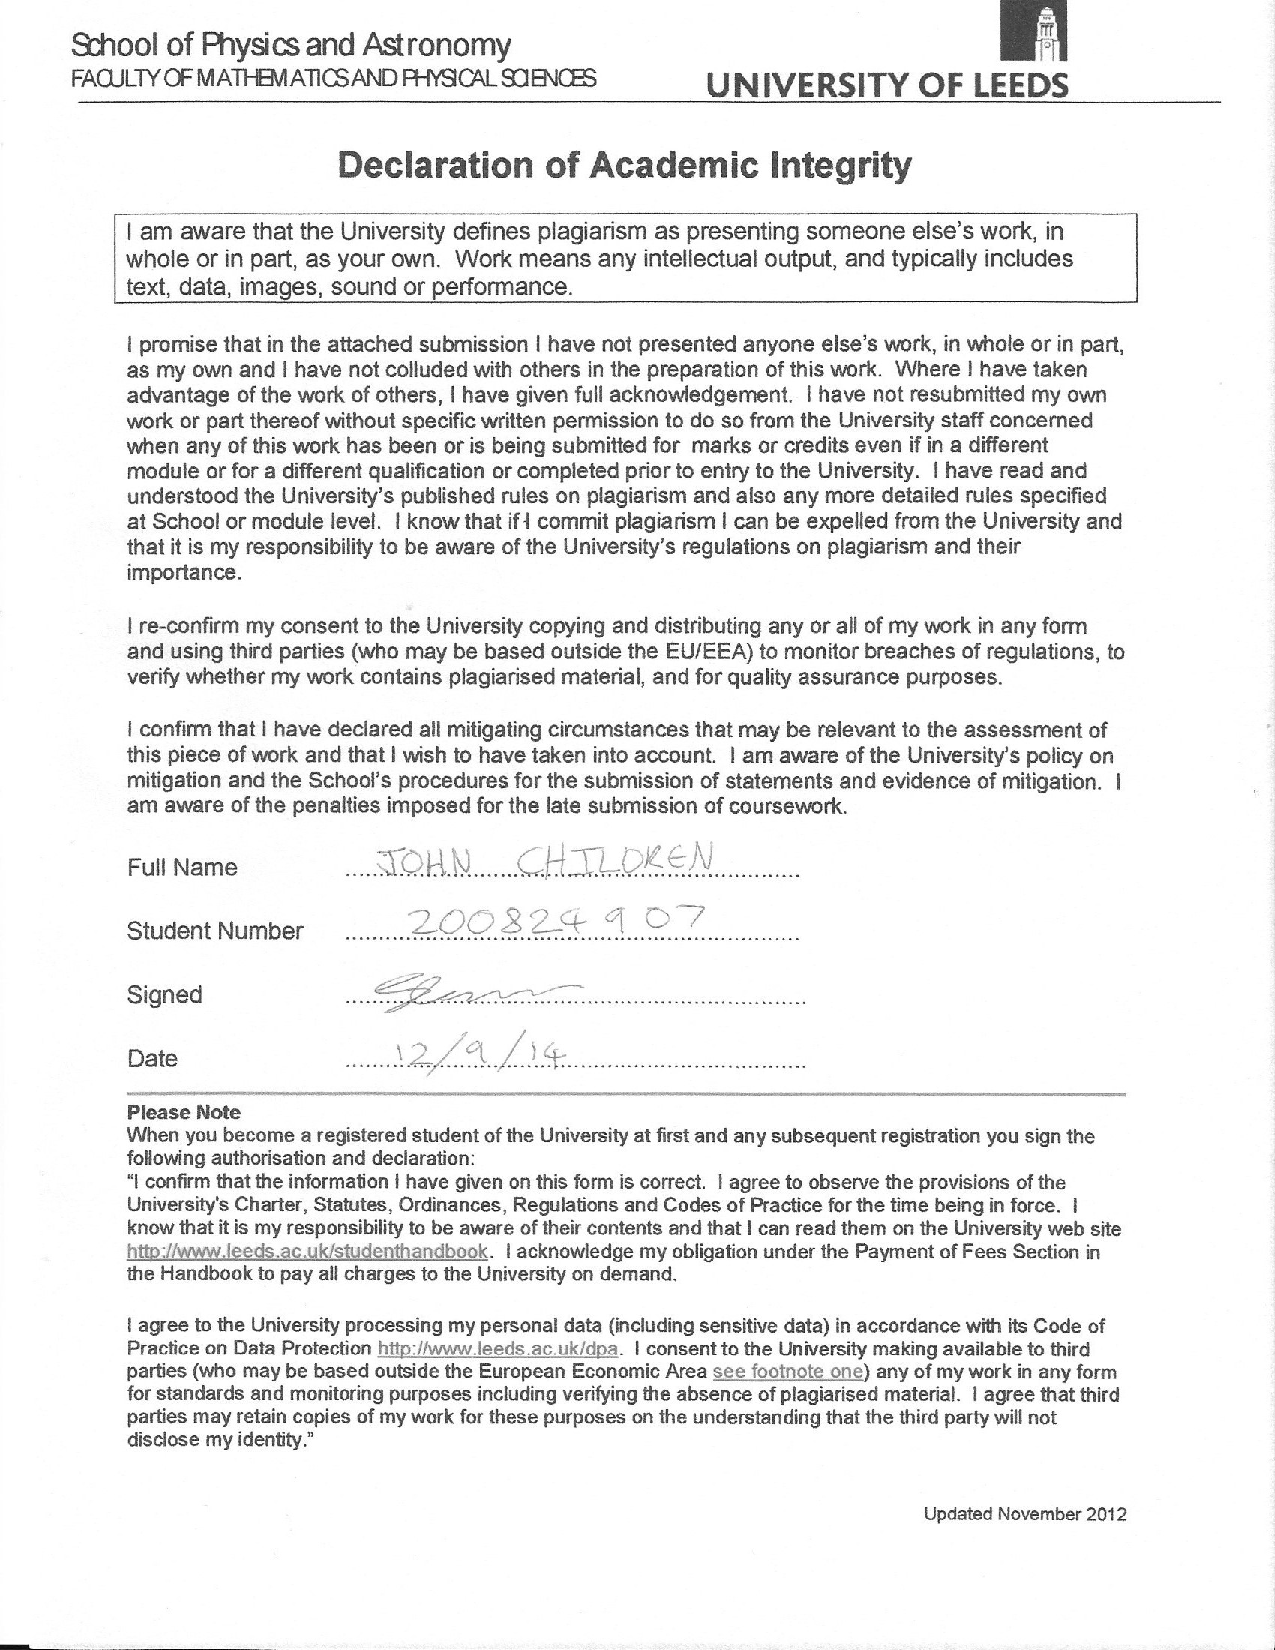
\includepdf{academicintegrity.pdf}

%\cleardoublepage% Dedication

\thispagestyle{empty}
\refstepcounter{dummy}

\pdfbookmark[1]{Dedication}{Dedication} % Bookmark name visible in a PDF viewer

\vspace*{3cm}

\begin{center}
\emph{Ohana} means family. \\
Family means nobody gets left behind, or forgotten. \\ \medskip
--- Lilo \& Stitch    
\end{center}

\medskip

\begin{center}
Dedicated to the loving memory of Rudolf Miede. \\ \smallskip
1939\,--\,2005
\end{center} % Dedication page

%\cleardoublepage\include{FrontBackMatter/Foreword} % Uncomment and create a Foreword.tex to include a foreword

% Abstract

\pdfbookmark[1]{Abstract}{Abstract} % Bookmark name visible in a PDF viewer

\begingroup
\let\clearpage\relax
\let\cleardoublepage\relax
\let\cleardoublepage\relax

\chapter*{Abstract} % Abstract name

We investigate one way quantum computation and an associated error correction scheme in order to build a numerical Monte Carlo model for fault tolerance for the model. Though the model is incomplete, we draw conclusions about difficulties in construction of the model and advise improvements that could be made to simulate the system accurately. \\

\textbf{Word count:} 15979

\endgroup			

\vfill % Abstract page

%\cleardoublepage% Publications - a page listing research articles written using content in the thesis

\pdfbookmark[1]{Publications}{Publications} % Bookmark name visible in a PDF viewer

\chapter*{Publications} % Publications page text

Some ideas and figures have appeared previously in the following publications:

\bigskip

\noindent Put your publications from the thesis here. The packages \texttt{multibib} or \texttt{bibtopic} etc. can be used to handle multiple different bibliographies in your document. % Publications from the thesis page

%\cleardoublepage% Acknowledgements

\pdfbookmark[1]{Acknowledgements}{Acknowledgements} % Bookmark name visible in a PDF viewer

\begin{flushright}{\slshape    
We have seen that computer programming is an art, \\ 
because it applies accumulated knowledge to the world, \\ 
because it requires skill and ingenuity, and especially \\
because it produces objects of beauty.} \\ \medskip
--- \defcitealias{knuth:1974}{Donald E. Knuth}\citetalias{knuth:1974} \citep{knuth:1974}
\end{flushright}

\bigskip

%----------------------------------------------------------------------------------------

\begingroup

\let\clearpage\relax
\let\cleardoublepage\relax
\let\cleardoublepage\relax

\chapter*{Acknowledgements} % Acknowledgements section text

Put your acknowledgements here.\\

\noindent Many thanks to everybody who already sent me a postcard!\\

\noindent Regarding the typography and other help, many thanks go to Marco Kuhlmann, Philipp Lehman, Lothar Schlesier, Jim Young, Lorenzo Pantieri and Enrico Gregorio\footnote{Members of GuIT (Gruppo Italiano Utilizzatori di \TeX\ e \LaTeX )}, J\"org Sommer, Joachim K\"ostler, Daniel Gottschlag, Denis Aydin, Paride Legovini, Steffen Prochnow, Nicolas Repp, Hinrich Harms, Roland Winkler,  and the whole \LaTeX-community for support, ideas and some great software.

\bigskip

\noindent\emph{Regarding \mLyX}: The \mLyX\ port was intially done by
\emph{Nicholas Mariette} in March 2009 and continued by
\emph{Ivo Pletikosi\'c} in 2011. Thank you very much for your work and the contributions to the original style.

\endgroup % Acknowledgements page

\pagestyle{scrheadings} % Show chapter titles as headings

% Table of Contents - List of Tables/Figures/Listings and Acronyms

\refstepcounter{dummy}

\pdfbookmark[1]{\contentsname}{tableofcontents} % Bookmark name visible in a PDF viewer

\setcounter{tocdepth}{2} % Depth of sections to include in the table of contents - currently up to subsections

\setcounter{secnumdepth}{3} % Depth of sections to number in the text itself - currently up to subsubsections

\manualmark
\markboth{\spacedlowsmallcaps{\contentsname}}{\spacedlowsmallcaps{\contentsname}}
\tableofcontents 
\automark[section]{chapter}
\renewcommand{\chaptermark}[1]{\markboth{\spacedlowsmallcaps{#1}}{\spacedlowsmallcaps{#1}}}
\renewcommand{\sectionmark}[1]{\markright{\thesection\enspace\spacedlowsmallcaps{#1}}}

\clearpage

\begingroup 
\let\clearpage\relax
\let\cleardoublepage\relax
\let\cleardoublepage\relax

%----------------------------------------------------------------------------------------
%	List of Figures
%----------------------------------------------------------------------------------------

%\refstepcounter{dummy}
\addcontentsline{toc}{chapter}{\listfigurename} % Uncomment if you would like the list of figures to appear in the table of contents
%\pdfbookmark[1]{\listfigurename}{lof} % Bookmark name visible in a PDF viewer

\listoffigures

%\vspace*{8ex}
\newpage

%----------------------------------------------------------------------------------------
%	List of Tables
%----------------------------------------------------------------------------------------

%\refstepcounter{dummy}
%\addcontentsline{toc}{chapter}{\listtablename} % Uncomment if you would like the list of tables to appear in the table of contents
%\pdfbookmark[1]{\listtablename}{lot} % Bookmark name visible in a PDF viewer

%\listoftables
        
%\vspace*{8ex}
%\newpage
    
%----------------------------------------------------------------------------------------
%	List of Listings
%---------------------------------------------------------------------------------------- 

%\refstepcounter{dummy}
\addcontentsline{toc}{chapter}{\lstlistlistingname} % Uncomment if you would like the list of listings to appear in the table of contents
%\pdfbookmark[1]{\lstlistlistingname}{lol} % Bookmark name visible in a PDF viewer

\lstlistoflistings 

%\vspace*{8ex}
%\newpage
    
                   
\endgroup % Contents, list of figures/tables/listings and acronyms

\pagenumbering{arabic} % Arabic page numbering for thesis content (1, 2, 3, etc)
%\setcounter{page}{90} % Uncomment to manually start the page counter at an arbitrary value (for example if you wish to count the pre-content pages in the page count)

\cleardoublepage % Avoids problems with pdfbookmark

%----------------------------------------------------------------------------------------
%	THESIS CONTENT - CHAPTERS
%----------------------------------------------------------------------------------------

% Chapter X

\chapter{Introduction and Background} % Chapter title

\label{ch:intro} % For referencing the chapter elsewhere, use \autoref{ch:name} 

The very first step in development of a numerical simulation for a one way quantum computer, is to define terms so that the accuracy of the model can be checked. To this aim, we first establish a definition of cluster states as well as the features of a measurement based quantum computer so that we can examine the functionality of the one way quantum computer.

%----------------------------------------------------------------------------------------


\section{Cluster States}

The main phenomenon enabling measurement based quantum computation is through the use of cluster states \citep{briegel_measurement-based_2009}. These states are formed of N qubits interacting with each other in arrays with a high 'persistency' of entanglement \citep{briegel_persistent_2000}. Persistency is defined in 'Persistent entanglement in arrays of interacting particles' as the minimum number of local measurements such that the state is completely disentangled for all measurement outcomes. This property means that measurements can be made on individual qubits in the state that will not entirely disentangle the state \citep{briegel_persistent_2000}, allowing information to be passed from one qubit to another. Additionally, the states are also said to be 'maximally connected' if they measurements on qubits in a set can project two seperate qubits into a pure Bell state \citep{briegel_persistent_2000}. This has the advantage of allowing easily teleportable states be produced through measurements on these cluster states.

These states are generally formed in either optical lattices \citep{joo_generating_2012} or from photons \citep{kiesel_experimental_2005, walther_experimental_2005}, though other implementations are possible \citep{briegel_measurement-based_2009}.

%----------------------------------------------------------------------------------------

\section{Measurement Based Quantum Computation}

The term 'measurement based quantum computer' refers to a whole class of quantum computer architectures that use measurements instead of unitary operators to process information \citep{jozsa_introduction_2005}. Unlike some other 'alternative' methods of quantum computation, such as quantum annealing devices, Measurement based quantum computers are both universal and do not suffer from as greatly from problems with decoherence as qubits are discarded after measurement \citep{jozsa_introduction_2005}. However, different challenges arise from the difficulty in forming the required states and then measuring specific qubits \citep{briegel_measurement-based_2009}. 

In the specific case of the one way quantum computer, using the two properties of cluster states mentioned earlier, it is possible to perform measurements on a 'lattice' of entangled particles in order to form a kind of quantum circuit that processes information \cite{raussendorf_one-way_2001} and this is illustrated in figure \ref{fig:one_way}. The exact functionality of these circuits will be shown in the next section.

\begin{figure}
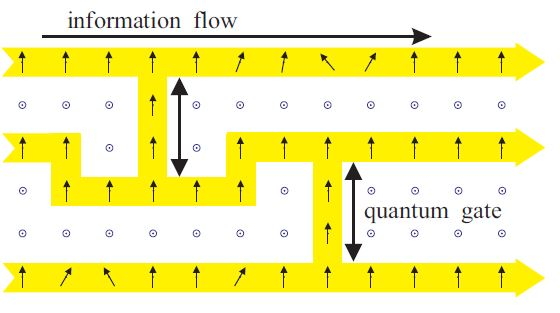
\includegraphics[scale=0.7]{gfx/infoflow.JPG}
\caption{Sketch of information flow in one way computation \citep{raussendorf_measurement-based_2003}}
\label{fig:one_way}
\end{figure}

 % Chapter 1
% Chapter X

\chapter{One Way Quantum Computation} % Chapter title

\label{ch:measurement} % For referencing the chapter elsewhere, use \autoref{ch:name} 

 In order to demonstrate how numerical simulation of one way quantum computation might be achieved, the first step is to examine the operation of the one way quantum computation. This involves examination of how cluster states can be formed as well as the function performed by measurement so that these procedures can be included in the simulation. In this regard, the procedures for functionality are detailed here so they might be compared to the program in later section to verify correct functionality.

%----------------------------------------------------------------------------------------

\section{Hamiltonian on interacting particles}
Following the work in 'Persistant Entanglement In Arrays of Interacting Particles', the Hamiltonian for a d-dimensional lattice at sites $a \in \mathbb{Z}^{d}$ interacting through short range interaction is \citep{briegel_persistent_2000}:

\begin{equation}
\label{eq:h_int}
\hat{H} _{int} = \hbar g(t) \sum\limits_{a, a'} f(a - a') \frac{1 - \sigma^{a}_{z}}{2} \frac{1 - \sigma^{a'}_{z}}{2}
\end{equation}

where:
\begin{align*}
f(a - a') &- \mbox{interaction range} \\
g(t) &- \mbox{time dependence of interaction} \\
\sigma_{z} &- \mbox{pauli-z operation}
\end{align*}

From the time dependent Schr\"{o}dinger equation we extract the time evolution of a wavefunction:

\begin{equation}
i\hbar \frac{\partial}{\partial t} \ket{\Psi} = \hat{H} \ket{\Psi}
\end{equation}

\begin{equation}
\ket{\Psi (t)} = e^{- \frac{i \hat{H} t}{\hbar}} \ket{\Psi (0)}
\end{equation}

From which we extract the time dependence operator:

\begin{equation}
\label{eq:td_op}
\hat{U} (t) = e^{- \frac{i \hat{H} t}{\hbar}}
\end{equation}

Substituting the interaction Hamiltonian \eqref{eq:h_int} into the time dependence operator\eqref{eq:td_op} gives:

\begin{equation}
\label{eq:td_op_h}
\hat{U} (t) = exp\left(-i g(t) t \sum\limits_{a, a'} f(a - a') \frac{1 - \sigma^{a}_{z}}{2} \frac{1 - \sigma^{a'}_{z}}{2}\right)
\end{equation}

Considering a one-dimensional chain of N-qubits with only next neighbour interactions the interaction range can be expressed as:

\begin{equation}
f(a - a') = \delta _{a + 1, a}
\end{equation}

Which will prevent qubits interacting with themselves and allow nearest neighbour interactions. Now we introduce a term $\phi$ which represents the integration of the time dependence of interaction such that:

\begin{equation}
\phi = \int g(t) \, dt = C g(t) t + D
\end{equation}

Where C and D are constants. Therefore the time evolution operator becomes

\begin{equation}
\label{eq:td_op_phi}
\hat{U} (t) = exp\left(-i \phi \sum\limits_{a} \frac{1 - \sigma^{a}_{z}}{2} \frac{1 - \sigma^{a + 1}_{z}}{2}\right)
\end{equation}

 

%------------------------------------------------

\section{Two qubit cluster state}

We can further refine this operator for the interaction between two qubits through the use of Euler's relation for operators:

\begin{equation}
\label{eq:euler}
e^{i  \theta \hat{A}} = \cos(\theta) \hat{\mathbb{1}} + i \sin (\theta) \hat{A}
\end{equation}

Now,we can expand the equation \eqref{eq:td_op_phi} as there are only two qubits to give:

\begin{equation}
\label{eq:td_op_phi_exp}
\hat{U} (t) = exp\left(-\frac{i \phi}{4} \left(\mathbb{1} \otimes \mathbb{1} - \mathbb{1} \otimes \sigma_{z} - \sigma_{z} \otimes \mathbb{1} + \sigma_{z} \otimes \sigma_{z} \right)\right)
\end{equation}

Typically we would need to apply the Baker-Campbell-Hausdorff formula to convert these terms into something more manageable, however the operators $\mathbb{1}$ and $\sigma_{z}$ are commutative, as are their tensor products, so all but the first two terms of the Baker-Campbell-Hausdorff expansion can be neglected leaving:

\begin{equation}
\hat{U} (t) = exp(-\frac{i \phi}{4} \mathbb{1} \otimes \mathbb{1})
exp(\frac{i \phi}{4} \sigma_{z} \otimes \mathbb{1})
exp(\frac{i \phi}{4} \sigma_{z} \otimes \mathbb{1}) 
exp(-\frac{i \phi}{4} \sigma_{z} \otimes \sigma_{z})
\end{equation}

Applying equation \eqref{eq:euler}:

\begin{multline}
\hat{U} (t) = exp(-\frac{i \phi \mathbb{1}}{4}) \\
\left(\cos(\frac{i \phi}{4}) \mathbb{1} \otimes \mathbb{1}
+ i \sin (\frac{i \phi}{4}) \mathbb{1} \otimes \sigma_{z}\right) \\
\left(\cos(\frac{i \phi}{4}) \mathbb{1} \otimes \mathbb{1}
+ i \sin (\frac{i \phi}{4}) \sigma_{z} \otimes \mathbb{1}\right) \\
\left(\cos(\frac{-i \phi}{4}) \mathbb{1} \otimes \mathbb{1}
+ i \sin (\frac{-i \phi}{4}) \sigma_{z} \otimes \sigma_{z}\right) \\
\end{multline}

In the case of $\phi = \pi$ this becomes:

\begin{multline}
\hat{U} (t) = \frac{1}{2 \sqrt{2}}exp(-\frac{i \pi}{4}) \mathbb{1} \\
\left( \mathbb{1} \otimes \mathbb{1}
+ i \mathbb{1} \otimes \sigma_{z}\right) \\
\left( \mathbb{1} \otimes \mathbb{1}
+ i \sigma_{z} \otimes \mathbb{1}\right) \\
\left( \mathbb{1} \otimes \mathbb{1}
- i \sigma_{z} \otimes \sigma_{z}\right) \\
\end{multline}

Now, expanding brackets and simplifying in two steps:

\begin{multline*}
\hat{U} (t) = \frac{1}{2 \sqrt{2}}exp(-\frac{i \pi}{4}) \mathbb{1} \\
\left( \mathbb{1} \otimes \mathbb{1}
- \sigma_{z} \otimes \sigma_{z}
+ i \mathbb{1} \otimes \sigma_{z}
+ i \sigma_{z} \otimes \mathbb{1} \right) \\
\left( \mathbb{1} \otimes \mathbb{1}
- i \sigma_{z} \otimes \sigma_{z}\right) \\ \\
 = \frac{1}{2 \sqrt{2}}exp(-\frac{i \pi}{4}) \\
( \mathbb{1} \otimes \mathbb{1}
- \sigma_{z} \otimes \sigma_{z}
+ i \mathbb{1} \otimes \sigma_{z}
+ i \sigma_{z} \otimes \mathbb{1} \\
+ i \mathbb{1} \otimes \mathbb{1}
- i \sigma_{z} \otimes \mathbb{z}
+ \mathbb{1} \otimes \sigma_{z}
+ \sigma_{z} \otimes \mathbb{1} ) \\
\end{multline*}

Factorising real and imaginary terms:

\begin{multline}
\label{eq:u_last_simp}
\hat{U} (t) = \frac{1}{2}
exp(-\frac{i \pi}{4}) 
\frac{1 + i}{\sqrt{2}} \\
\left( \mathbb{1} \otimes \mathbb{1}
- \sigma_{z} \otimes \sigma_{z}
+ \mathbb{1} \otimes \sigma_{z}
+ \sigma_{z} \otimes \mathbb{1}\right) \\
\end{multline}

As $exp(-\frac{i \pi}{4}) = \frac{1 - i}{\sqrt{2}}$ equation \eqref{eq:u_last_simp} simplifies to:

\begin{multline}
\label{eq:u_final}
\hat{U} (t) = \frac{1}{2}
\left( \mathbb{1} \otimes \mathbb{1}
+ \mathbb{1} \otimes \sigma_{z}
+ \sigma_{z} \otimes \mathbb{1}
- \sigma_{z} \otimes \sigma_{z}\right) \\
\end{multline}

If this operator is applied to two qubits in the $\ket{+ +}$ state, for example, we get:

\begin{multline}
\label{eq:2qubit_example}
\hat{U} (t) \ket{+ +} = \frac{1}{2}
(\ket{++} + \ket{+-} + \ket{-+} - \ket{--}) \\ \\
= \frac{1}{\sqrt{2}} (\ket{+ 0} + \ket{- 1}) \\
\end{multline}

%------------------------------------------------

\section{Three qubit cluster state}

By using the same method used in the previous section, we can also obtain a the time evolution operator for a chain of three qubits only interacting with their nearest neighbour. In this case the time evolution operator will be

\begin{equation}
\hat{U} (t) = exp\left(-i \phi \left( 
\frac{1 - \sigma^{1}_{z}}{2} \frac{1 - \sigma^{2}_{z}}{2}\mathbb{1}
+ \mathbb{1}\frac{1 - \sigma^{2}_{z}}{2} \frac{1 - \sigma^{3}_{z}}{2}
\right)\right)
\end{equation}

Expanding out this expression gives:

\begin{multline}
\hat{U} (t) = exp(-\frac{i \phi}{4}( 
2 \mathbb{1} \otimes \mathbb{1} \otimes \mathbb{1}
- 2 \mathbb{1} \otimes \sigma_{z} \otimes \mathbb{1} \\
- \sigma_{z} \otimes \mathbb{1} \otimes \mathbb{1}
- \mathbb{1} \otimes \mathbb{1} \otimes \sigma_{z} \\
+ \sigma_{z} \otimes \sigma_{z} \otimes \mathbb{1}
+ \mathbb{1} \otimes \sigma_{z} \otimes \sigma_{z} 
)) \\
\end{multline}

Applying Baker-Campbell-Hausdorff and Euler's rule:

\begin{multline*}
\hat{U} (t) = exp(-\frac{i \phi}{2}) \\
\left(\cos(\frac{i \phi}{2}) \mathbb{1} \otimes \mathbb{1} \otimes \mathbb{1}
+ i \sin (\frac{i \phi}{2}) \mathbb{1} \otimes \sigma_{z} \otimes \mathbb{1}\right) \\
\left(\cos(\frac{i \phi}{4}) \mathbb{1} \otimes \mathbb{1} \otimes \mathbb{1}
+ i \sin (\frac{i \phi}{4}) \sigma_{z} \otimes \mathbb{1} \otimes \mathbb{1}\right) \\
\left(\cos(\frac{i \phi}{4}) \mathbb{1} \otimes \mathbb{1} \otimes \mathbb{1}
+ i \sin (\frac{i \phi}{4}) \mathbb{1} \otimes \mathbb{1} \otimes \sigma_{z}\right) \\
\left(\cos(\frac{-i \phi}{4}) \mathbb{1} \otimes \mathbb{1} \otimes \mathbb{1}
+ i \sin (\frac{-i \phi}{4}) \sigma_{z} \otimes \sigma_{z} \otimes \mathbb{1}\right) \\
\left(\cos(\frac{-i \phi}{4}) \mathbb{1} \otimes \mathbb{1} \otimes \mathbb{1}
+ i \sin (\frac{-i \phi}{4}) \mathbb{1} \otimes \sigma_{z} \otimes \sigma_{z}\right) \\
\end{multline*}

Once again, using $\phi = \pi$, we expand the terms of the equation and simplify

\begin{multline*}
\hat{U} (t) = exp(-\frac{i \pi}{2})
(i \mathbb{1} \otimes \sigma_{z} \otimes \mathbb{1}) \\
(\mathbb{1} \otimes \mathbb{1} \otimes \mathbb{1} + i \sigma_{z} \otimes \mathbb{1} \otimes \mathbb{1})
(\mathbb{1} \otimes \mathbb{1} \otimes \mathbb{1} + i \mathbb{1} \otimes \mathbb{1} \otimes \sigma_{z}) \\
(\mathbb{1} \otimes \mathbb{1} \otimes \mathbb{1} - i \sigma_{z} \otimes \sigma_{z} \otimes \mathbb{1})
(\mathbb{1} \otimes \mathbb{1} \otimes \mathbb{1} - i \mathbb{1} \otimes \sigma_{z} \otimes \sigma_{z}) \\ \\
= exp(-\frac{i \pi}{2}) (i \mathbb{1} \otimes \sigma_{z} \otimes \mathbb{1}) \\
(\mathbb{1} \otimes \mathbb{1} \otimes \mathbb{1}
+ i \sigma_{z} \otimes \mathbb{1} \otimes \mathbb{1}
+ i \mathbb{1} \otimes \mathbb{1} \otimes \sigma_{z}
- \sigma_{z} \otimes \mathbb{1} \otimes \sigma_{z}) \\
(\mathbb{1} \otimes \mathbb{1} \otimes \mathbb{1}
- i \sigma_{z} \otimes \sigma_{z} \otimes \mathbb{1}
- i \mathbb{1} \otimes \sigma_{z} \otimes \sigma_{z}
+ \sigma_{z} \otimes \mathbb{1} \otimes \sigma_{z}) \\ \\
= exp(-\frac{i \pi}{2}) (i \mathbb{1} \otimes \sigma_{z} \otimes \mathbb{1}) \\ 
(\mathbb{1} \otimes \mathbb{1} \otimes \mathbb{1}
- i \mathbb{1} \otimes \sigma_{z} \otimes \sigma_{z}
- i \sigma_{z} \otimes \sigma_{z} \otimes \mathbb{1}
- \sigma_{z} \otimes \mathbb{1} \otimes \sigma_{z}
+ i \sigma_{z} \otimes \mathbb{1} \otimes \mathbb{1} \\
+ \sigma_{z} \otimes \sigma_{z} \otimes \sigma_{z}
+ \mathbb{1} \otimes \sigma_{z} \otimes \mathbb{1}
- i \mathbb{1} \otimes \mathbb{1} \otimes \sigma_{z}
+ i \mathbb{1} \otimes \mathbb{1} \otimes \sigma_{z} \\
+ \mathbb{1} \otimes \sigma_{z} \otimes \mathbb{1}
+ \sigma_{z} \otimes \sigma_{z} \otimes \sigma_{z}
- i \sigma_{z} \otimes \sigma_{z} \otimes \mathbb{1} 
- \sigma_{z} \otimes \mathbb{1} \otimes \sigma_{z} \\
+ i \sigma_{z} \otimes \sigma_{z} \otimes \mathbb{1}
+ i \mathbb{1} \otimes \sigma_{z} \otimes \sigma_{z}
+ \sigma_{z} \otimes \sigma_{z} \otimes \sigma_{z}) \\
\end{multline*}

Many of these terms will cancel and as $\frac{1}{2} exp(-\frac{i \pi}{2}) = \frac{i}{2}$ we are left with:

\begin{equation}
\label{eq:u_final3}
\hat{U} = \frac{1}{2}(
  \mathbb{1} \otimes \mathbb{1} \otimes \mathbb{1}
+ \mathbb{1} \otimes \sigma_{z} \otimes \mathbb{1} 
+ \sigma_{z} \otimes \mathbb{1} \otimes \sigma_{z}
- \sigma_{z} \otimes \sigma_{z} \otimes \sigma_{z}
)
\end{equation}

Applying this to the state $\ket{+ + +}$:

\begin{equation}
\label{eq:3plus_2cz}
\hat{U} \ket{+ + +}= \frac{1}{\sqrt{2}}(\ket{+0+} + \ket{-1-})
\end{equation}

However, we could have quite simply achieved the result from equation \eqref{eq:u_final3} by applying equation \eqref{eq:u_final} twice to the three qubits. This is due to the nature of the interaction Hamiltonian being used and as such we can consider all links between two qubits to have this same property and as such we can construct time evolution operators for any system using this operator as a building block. This can be demonstrated by applying the unitary operator \eqref{eq:u_final} to the state described in \eqref{eq:2qubit_example} and an addition $\ket{+}$ state.

\begin{multline}
\frac{1}{2}
\left( \mathbb{1}_{2} \otimes \mathbb{1}_{3}
+ \mathbb{1}_{2} \otimes \sigma_{z3}
+ \sigma_{z2} \otimes \mathbb{1}_{3}
- \sigma_{z2} \otimes \sigma_{z3}\right) 
\frac{1}{\sqrt{2}} (\ket{+ 0} + \ket{- 1}) \ket{+}\\
= \frac{1}{2\sqrt{2}} (\ket{+}(\ket{0 +} + \ket{0 -} + \ket{0 +} - \ket{0 -}) \\
 + \ket{-}(\ket{1 -} + \ket{1 +} - \ket{1 -} + \ket{1 +}))\\
= \frac{1}{\sqrt{2}} (\ket{+ 0 +} + \ket{- 1 -}) \\
\end{multline}

Hence CZ operators can be applied in sequence to form cluster states of any desired size or topology. This will be utilised later in the programming stage when creating subroutines to handle the initialisation of the system.

%----------------------------------------------------------------------------------------

\section{Quantum controlled Z operator}

Consider a 2 qubit state prepared as $\ket{+ +}$ and subject to the unitary transform \eqref{eq:u_final} for two qubit cluster states:

\begin{multline*}
\hat{U} \ket{+ +} = \frac{1}{\sqrt{2}} (\ket{+ 0} + \ket{- 1}) \\
=  \frac{1}{2} (\ket{0 0} + \ket{0 1} + \ket{1 0} - \ket{1 1}) \\
= \frac{1}{2} \begin{pmatrix}
1 \\
1 \\
1 \\
-1
\end{pmatrix} \\
\end{multline*}

As the matrix expression for $\ket{+ +}$ is:

\begin{equation}
\ket{+ +} = 
\frac{1}{2} \begin{pmatrix}
1 \\
1 \\
1 \\
1
\end{pmatrix} \\
\end{equation}

So the transformation matrix between the two is:

\begin{equation}
\begin{pmatrix}
1 & 0 & 0 & 0 \\
0 & 1 & 0 & 0 \\
0 & 0 & 1 & 0 \\
0 & 0 & 0 & -1 \\
\end{pmatrix}
\end{equation}

Which can be expressed as a unitary transform that forms a conditional phase gate between qubits a and b.

\begin{equation}
S^{ab} = \ket{0}_{a} \bra{0} \otimes \mathbb{1}^{b} + \ket{1}_{a} \bra{1} \otimes \sigma_{z}^{b}
\end{equation}

Therefore the unitary operator is equivalent to the CZ operation in the circuit model. In general we can perform a controlled phase operation in the z axis in a similar form:

\begin{equation}
\begin{pmatrix}
1 & 0 & 0 & 0 \\
0 & 1 & 0 & 0 \\
0 & 0 & 1 & 0 \\
0 & 0 & 0 & e^{-i \alpha} \\
\end{pmatrix}
\end{equation}

Where $\alpha$ is the phase of the operation.


%----------------------------------------------------------------------------------------

\section{Measurement based gate operation}

The basic principle of computation in the one way quantum computer follows three simple steps. The first step involves the formation of a cluster state through the use of the CZ operation demonstrated earlier. The next step involves measurement of the state of specific qubits in a particular measurement basis depending upon the computational operation required. Finally, the outcomes of measurement are fed forward in order to determine the result of computation when the output is measured. Therefore we shall next examine the types of measurements required to achieve quantum computation through this method.

%----------------------------------------------------------------------------------------

\subsection{One bit teleportation}

The most simple kind of operation that can be performed in one way quantum computation is through the use of teleportation to transfer the state of one qubit so that the information of the state can be projected to the other through applying measurements with a particular basis to the first qubit. To demonstrate this in general we can consider a qubit in unknown state $\ket{\psi}_{1} = a \ket{0}_{1} + b \ket{1}_{1}$ and second qubit in state $\ket{+}$. 

\begin{equation}
\ket{\psi}_{1} \otimes \ket{+}_{2} = (a \ket{0}_{1} + b \ket{1}_{1}) \frac{1}{\sqrt{2}} (\ket{0}_{1} + \ket{1}_{1})
\end{equation}

A CZ operation is applied to qubit 1 and 2 such that they become entangled similarly to the two qubit $+$ state in \eqref{eq:2qubit_example}.

\begin{multline}
CZ_{12}\ket{\psi}_{12} = \frac{1}{\sqrt{2}} (a \ket{00}_{12} + a \ket{01}_{12} + \ket{10}_{12} - b \ket{11}_{12}) \\
= (a \ket{0+}_{12} + b \ket{1-}_{12}) \\
\end{multline}

The first qubit is then measured in a basis corresponding to it's phase angle. 

\begin{equation}
\hat{M} = \set{ \ket{+ \psi} \bra{+ \psi}, \ket{- \psi} \bra{- \psi}}
\end{equation}

There are two possible measurement outcomes $\ket{+ \psi}_{1}$ and $\ket{- \psi}_{2}$ that can result here. In the first case of $\ket{+ \psi}_{1}$.

\begin{multline}
\ket{+ \psi}_{1} \frac{1}{\sqrt{2}} (\bra{0}_{1} + e^{-i \psi} \bra{1}_{1}) (a \ket{0+}_{12} + b \ket{1-}_{12}) \\
= \ket{+ \psi}_{1} [\braket{0|0}_{1} a \ket{+}_{2} + e^{-i \psi} \braket{1|1}_{1} b \ket{-}_{2}] \\
= \frac{1}{\sqrt{2}} \ket{+ \psi}_{1} (a \ket{+}_{2} + e^{-i \psi} b \ket{-}_{2}) \\
\end{multline}

The information contained in the phase of the original qubit can then be obtained through the application of a series of operations which will project the information state onto the second qubit.

\begin{multline}
\ket{out^{0}}_{2} = a \ket{+}_{2} + b e^{-i \psi} \ket{-}_{2} \\
= H_{2} (a \ket{0}_{2} + b e^{-i \psi} \ket{1}_{2}) \\
= e^{\frac{-i \psi}{2}} H R_{z} (-\psi) (a \ket{0}_{2} + b \ket{1}_{2}) \\
\end{multline}

However, when the opposite measurement outcome occurs, the state will be projected such that an X operation is also required. 

\begin{multline}
\ket{out^{1}}_{2} = X_{2} (a \ket{+} + b e^{-i \psi} \ket{-}) \\
= X_{2} \ket{out^{0}}_{2} \\
\end{multline}

Thus in general we can recover the information projected onto one qubit through the measurement of two qubits entangled by a CZ operation through the following operations:

\begin{equation}
\label{eq:one_qbit_feed_forward}
\ket{out^{m_{i}}}_{2} = e^{\frac{-i \psi}{2}} X^{m_{i}} H R_{z} (-\psi) (a \ket{0}_{2} + b \ket{1}_{2}) 
\end{equation}

Where $m_{i}$ represents the number of the basis used in measurement. 

%----------------------------------------------------------------------------------------

\subsection{Controlled not gate}

In order to form a CNOT gate however, at least two qubits are required so the generalised rotation shown in the previous section is not sufficient. Therefore a new geometry is required which forms a T-shape consisting of four qubits. On the left end of longer side of the shape we have our target qubit in a particular state $\ket{\psi_{T}}$ and on the bottom of the shape is the control qubit $\ket{\phi_{c}}$. The relationship between the states of these two qubits is such that the intended output will be:

\begin{multline}
\label{eq:cnot}
CNOT_{14} \ket{\psi_{T}} \ket{\phi_{C}} = CNOT_{14} (a \ket{0}_{1} + b \ket{1}_{1}) (c \ket{0}_{4} + d \ket{1}_{4}) \\
= ac \ket{00}_{14} + bd \ket{01}_{14} + bc \ket{10} + ad \ket{11}_{14} \\
\end{multline}

In order to prepare the qubits for measurement we prepare a state $\ket{\psi^{in}}$ that denotes the input state of the qubits formed of multiple CZ operations in order to create our T-shape of entanglement. By applying CZ operations to the known initial states of our four qubits we can determine how this state is represented to find the results of measurements.

\begin{multline}
\ket{\psi^{in}} = CZ_{12} CZ_{23} CZ_{24} \ket{\psi_{T}}_{1} \ket{+}_{2} \ket{+}_{3} \ket{\phi_{4}} \\
= CZ_{21} CZ_{32} CZ_{24} \ket{\psi_{T}}_{1} \ket{+}_{2} \ket{+}_{3} \ket{\phi_{4}} \\
= \frac{1}{2} (\ket{\psi_{T}}_{1} (\ket{0}_{2} + \ket{1}_{2} Z_{1}) (\ket{0}_{3} + \ket{1}_{3} Z_{2}) (c \ket{0}_{3} + d \ket{1}_{3} Z_{3}) \\
= \frac{1}{2} ((\ket{\psi_{T}}_{1} \ket{0}_{2} + \ket{\psi_{T}}_{1} \ket{1}_{2} Z_{1}) \\ (\ket{0}_{3} + \ket{1}_{3} Z_{2}) (c \ket{0}_{3} + d \ket{1}_{3} Z_{3}) \\
= \frac{1}{2} (\ket{\psi_{T}}_{1} \ket{00}_{23} + Z_{1} \ket{\psi_{T}}_{1} \ket{01}_{23} \\
- (Z_{2} \ket{\psi_{T}}_{1} \ket{10}_{23} - Z_{1} \ket{\psi_{T}}_{1} \ket{11}_{23})(c \ket{0}_{4} + d \ket{1}_{4} Z_{3}) \\
= \frac{1}{\sqrt{2}}(\ket{\psi_{T}}_{1} \ket{0}_{2} \ket{+}_{3} \ket{\phi_{c}}_{4}+ (Z_{1} \ket{\psi_{T}}_{1}) \ket{1}_{2} \ket{-}_{3} (Z_{3} \ket{\phi_{c}}_{4}) \\
\end{multline}

In order to perform a CNOT operation using this state between the target and control qubits we then measure qubits 1 and 2 in the basis $\set{\ket{+}, \ket{-}}$. In the case of $\ket{+}$ measurement this results in:

\begin{multline}
_{1} \braket{+ | \psi^{in}}_{1234} = \frac{1}{\sqrt{2}} ((a + b) \ket{0}_{2} \ket{+}_{3} \ket{\phi_{c}}_{4} \\
 + (a-b) \ket{1}_{2} \ket{-}_{4} (Z_{4} \ket{\phi_{c}}_{4}))
\end{multline}

This state then becomes:

\begin{multline}
(\ket{+} \otimes \ket{+}) \bra{\psi^{in}}_{1234} ac \ket{00}_{34} + bd \ket{01}_{34} + bc \ket{10}_{34} + ad \ket{11}_{34} \\
= \ket{out}_{34}
\end{multline}

Which from equation \eqref{eq:cnot} we can see is in fact the desired CNOT with some additional operators applied. Therefore in order to recover correct output we feed forward measurement outputs for the first two qubits to obtain the output:

\begin{equation}
\label{eq:CNOT_qbit_feed_forward}
\ket{out^{m_{1} m_{2}}} = X^{n_{2}}_{T} Z^{n_{1}}_{T} X^{n_{1}}_{C} CNOT \ket{\psi_{T}}_{3} \ket{\phi_{C}}_{4}
\end{equation}

%----------------------------------------------------------------------------------------

\subsection{Gate universality}

The two gate operations here can be used to form a universal set of gates \citep{raussendorf_quantum_2000}. This set can be expressed analogously to the more commonly used universal set of five gates in the circuit model, which is demonstrated in \citep{raussendorf_measurement-based_2003} and shown in Figure \ref{fig:universal_set}. Therefore, if we can simulate these two gates as described here we can simulate any possible measurement based gate. 

\begin{figure}
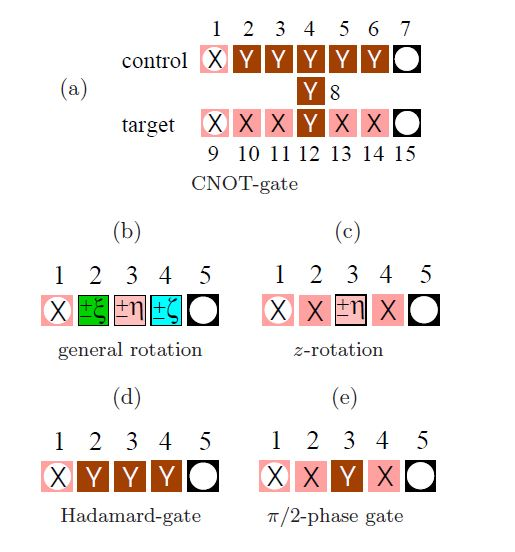
\includegraphics[scale=0.8]{gfx/gates.JPG}
\caption{Universal set of quantum gates \citep{raussendorf_measurement-based_2003}}
\label{fig:universal_set}
\end{figure} % Chapter 2
% Chapter X

\chapter{Error Correction} % Chapter title

\label{ch:name} % For referencing the chapter elsewhere, use \autoref{ch:name} 

The next part of the simulation will be the error correction scheme. In order to keep the program initially as simple as possible a variant of Jaewoo Joo's measurement based error correction scheme  using two auxilary qubits to create a 'triangle state' instead of the 'pentagon state's used in Joo's paper \citep{joo_error-correcting_2009}. This error correction scheme is convenient as it can be extended to larger size logical qubits easily so the correlation between fault tolerance and qubit number can be examined.

%----------------------------------------------------------------------------------------

\section{Logical qubits}

The first step towards simulation of the error correction scheme for measurement based quantum computation requires the definition of a logical state which represents a quantum state for which the information is distributed amongst multiple qubits. Following the work in 'Error - correcting one - way quantum computation with global entangling gates' \citep{joo_error-correcting_2009} we establish a logical state based on three qubits, rather than the five in the paper, to form a triangle state through three CZ operations. In doing so we obtain the unitary operator that will allow for conversion of three qubits in the  + state to the logical + state.

\begin{multline}
\hat{U} (t) =
exp\Bigg(-i \phi \bigg( 
\frac{1 - \sigma^{1}_{z}}{2} \frac{1 - \sigma^{2}_{z}}{2}\mathbb{1} \\
+ \frac{1 - \sigma^{1}_{z}}{2} \mathbb{1} \frac{1 - \sigma^{3}_{z}}{2}
+ \mathbb{1}\frac{1 - \sigma^{2}_{z}}{2} \frac{1 - \sigma^{3}_{z}}{2}
\bigg)\Bigg) \\
\end{multline}

Expanding out this expression gives:

\begin{multline}
\hat{U} (t) = exp(-\frac{i \phi}{4}( 
3 \mathbb{1} \otimes \mathbb{1} \otimes \mathbb{1}
- 2 \mathbb{1} \otimes \sigma_{z} \otimes \mathbb{1} \\
- 2 \sigma_{z} \otimes \mathbb{1} \otimes \mathbb{1}
- 2 \mathbb{1} \otimes \mathbb{1} \otimes \sigma_{z} \\
+ \sigma_{z} \otimes \sigma_{z} \otimes \mathbb{1}
+ \mathbb{1} \otimes \sigma_{z} \otimes \sigma_{z} \\
+ \sigma_{z} \otimes \mathbb{1} \otimes \sigma_{z}
)) \\
\end{multline}

Applying Baker-Campbell-Hausdorff and Euler's rule:

\begin{multline*}
\hat{U} (t) = exp(-\frac{-3 i \phi}{4}) \\
\left(\cos(\frac{i \phi}{2}) \mathbb{1} \otimes \mathbb{1} \otimes \mathbb{1}
+ i \sin (\frac{i \phi}{2}) \mathbb{1} \otimes \sigma_{z} \otimes \mathbb{1}\right) \\
\left(\cos(\frac{i \phi}{2}) \mathbb{1} \otimes \mathbb{1} \otimes \mathbb{1}
+ i \sin (\frac{i \phi}{2}) \sigma_{z} \otimes \mathbb{1} \otimes \mathbb{1}\right) \\
\left(\cos(\frac{i \phi}{2}) \mathbb{1} \otimes \mathbb{1} \otimes \mathbb{1}
+ i \sin (\frac{i \phi}{2}) \mathbb{1} \otimes \mathbb{1} \otimes \sigma_{z}\right) \\
\left(\cos(\frac{-i \phi}{4}) \mathbb{1} \otimes \mathbb{1} \otimes \mathbb{1}
+ i \sin (\frac{-i \phi}{4}) \sigma_{z} \otimes \sigma_{z} \otimes \mathbb{1}\right) \\
\left(\cos(\frac{-i \phi}{4}) \mathbb{1} \otimes \mathbb{1} \otimes \mathbb{1}
+ i \sin (\frac{-i \phi}{4}) \mathbb{1} \otimes \sigma_{z} \otimes \sigma_{z}\right) \\
\left(\cos(\frac{-i \phi}{4}) \mathbb{1} \otimes \mathbb{1} \otimes \mathbb{1} 
+ i \sin (\frac{-i \phi}{4}) \sigma_{z} \otimes \mathbb{1} \otimes \sigma_{z}\right) \\
\end{multline*}

Using $\phi = \pi$, we expand the terms of the equation and simplify

\begin{multline*}
\hat{U} (t) = \frac{1}{2 \sqrt{2}}exp(-\frac{-3 i \pi}{4})
(i \mathbb{1} \otimes \sigma_{z} \otimes \mathbb{1}) \\
(i \mathbb{1} \otimes \mathbb{1} \otimes \sigma_{z}) \\
(i \sigma_{z} \otimes \mathbb{1} \otimes \mathbb{1}) \\
(\mathbb{1} \otimes \mathbb{1} \otimes \mathbb{1} - i \mathbb{1} \otimes \sigma_{z} \otimes \sigma_{z})
(\mathbb{1} \otimes \mathbb{1} \otimes \mathbb{1} - i \sigma_{z} \otimes \mathbb{1} \otimes \sigma_{z}) \\
(\mathbb{1} \otimes \mathbb{1} \otimes \mathbb{1} - i \sigma_{z} \otimes \sigma_{z} \otimes \mathbb{1}) \\ \\
= \frac{1}{2 \sqrt{2}}exp(-\frac{-3 i \pi}{4})
(i \sigma_{z} \otimes \sigma_{z} \otimes \sigma_{z}) \\
(\mathbb{1} \otimes \mathbb{1} \otimes \mathbb{1}
- i \sigma_{z} \otimes \mathbb{1} \otimes \sigma_{z}
- i \mathbb{1} \otimes \sigma_{z} \otimes \sigma_{z}
- \sigma_{z} \otimes \sigma_{z} \otimes \mathbb{1}) \\
(\mathbb{1} \otimes \mathbb{1} \otimes \mathbb{1} - i \sigma_{z} \otimes \sigma_{z} \otimes \mathbb{1}) \\ \\
= \frac{1}{2 \sqrt{2}}exp(-\frac{-3 i \pi}{4})
(i \sigma_{z} \otimes \sigma_{z} \otimes \sigma_{z}) \\
(\mathbb{1} \otimes \mathbb{1} \otimes \mathbb{1}
+ i \mathbb{1} \otimes \mathbb{1} \otimes \mathbb{1} \\
- \sigma_{z} \otimes \sigma_{z} \otimes \mathbb{1}
- i \sigma_{z} \otimes \sigma_{z} \otimes \mathbb{1} \\
- \sigma_{z} \otimes \mathbb{1} \otimes \sigma_{z} 
- i \sigma_{z} \otimes \mathbb{1} \otimes \sigma_{z} \\
- \mathbb{1} \otimes \sigma_{z} \otimes \sigma_{z}
- i \mathbb{1} \otimes \sigma_{z} \otimes \sigma_{z} \\ \\
= \frac{1 - i}{2 \sqrt{2}}exp(-\frac{-3 i \pi}{4})
(\mathbb{1} \otimes \mathbb{1} \otimes \sigma_{z}
+ \sigma_{z} \otimes \mathbb{1} \otimes \mathbb{1} \\
+ \mathbb{1} \otimes \sigma_{z} \otimes \mathbb{1}
- \sigma_{z} \otimes \sigma_{z} \otimes \sigma_{z}) \\
\end{multline*}

As $exp(-\frac{-3 i \pi}{4}) = - \frac{1 + i}{\sqrt{2}}$ we are left with:

\begin{equation}
\label{eq:u_final3_l}
\hat{U} \ket{+ + +}= \frac{1}{2}
(\mathbb{1} \otimes \mathbb{1} \otimes \sigma_{z}
+ \sigma_{z} \otimes \mathbb{1} \otimes \mathbb{1} \\
+ \mathbb{1} \otimes \sigma_{z} \otimes \mathbb{1}
- \sigma_{z} \otimes \sigma_{z} \otimes \sigma_{z}) \\
\end{equation}

Applying this to the state $\ket{+ + +}$:

\begin{equation}
\label{eq:logical3plus_u}
\hat{U}\ket{+ + +} = \frac{1}{2}(\ket{+-+} +\ket{++-} + \ket{-++} - \ket{---})
\end{equation}

This allows us to find our logical plus state by applying the operator to three qubits in the plus state to form our 'triangle state'.

\begin{equation}
\ket{+^{L}} = CZ_{12} CZ_{23} CZ_{13} \ket{+++}
\end{equation}

Applying the CZ operators in sequence:

\begin{multline*}
\ket{+^{L}} = \frac{1}{2} CZ_{23} CZ_{13}
(\ket{+++} + \ket{+-+} + \ket{-++} - \ket{--+}) \\ \\
= \frac{1}{2} CZ_{23} CZ_{13} (\ket{+}(\ket{++} + \ket{-+}) + \ket{-}(\ket{++} - \ket{-+})) \\ \\
= \frac{1}{4} CZ_{13} (\ket{+}(\ket{++} + \ket{+-} + \ket{-+} - \ket{--} 
\\+ \ket{-+} + \ket{++} + \ket{--} -\ket{+-})\\
+ \ket{-}(\ket{++} + \ket{+-} + \ket{-+} -\ket{--} - \ket{-+} 
\\- \ket{++} - \ket{--} + \ket{+-})) \\ \\
= \frac{1}{2} CZ_{13} (\ket{+}(\ket{++} + \ket{-+}) + \ket{-}(\ket{+-} - \ket{--})) \\ \\
= \frac{\sqrt{2}}{2} CZ_{13} (\ket{+0+} + \ket{-1-}) \\
\end{multline*}

Which is the result from \eqref{eq:3plus_2cz} with an additional CZ operation. Continuing by applying the final operator:

\begin{multline*}
\ket{+^{L}} = \frac{\sqrt{2}}{4}(\ket{+0+} + \ket{+0-} + \ket{-0+} - \ket{-0-} \\
 + \ket{-1-} + \ket{+1-} + \ket{-1+} - \ket{+1+}) \\
\end{multline*}

Which simplifies to:

\begin{equation}
\label{eq:logical3plus_cz}
\ket{+^{L}} = \frac{1}{2}(\ket{+-+} +\ket{++-} + \ket{-++} - \ket{---})
\end{equation}

So states \eqref{eq:logical3plus_u} and \eqref{eq:logical3plus_cz} are identical and applying three CZ operators to form a logical qubits is valid. By a similar method we can find that:  

\begin{equation}
\ket{-^{L}} = \frac{1}{2}(\ket{+++} - \ket{--+} - \ket{-+-} - \ket{+--})
\end{equation}

Then, by using the relations $\ket{0^{L}} = \frac{\ket{+^{L}} + \ket{-^{L}}}{\sqrt{2}}$ and $\ket{1^{L}} = \frac{\ket{+^{L}} - \ket{-^{L}}}{\sqrt{2}}$ we can find expressions for $\ket{0^{L}}$ and $\ket{1^{L}}$

\begin{equation}
\ket{0^{L}} = \frac{1}{2} (\ket{0++} - \ket{0--} + \ket{1+-} + \ket{1-+})
\end{equation}

\begin{equation}
\ket{1^{L}} = \frac{1}{2} (\ket{0+-} - \ket{1++} + \ket{1--} + \ket{0-+})
\end{equation}

But in order to use these qubits in computation we must first determine the equivalent logical gate operations.

%----------------------------------------------------------------------------------------

\section{Logical operations}

Logical gate operators represent the product of standard one qubit operations that transform one logical state into the other. Now that we have the four primary logical states that will be used for the model, we can determine the logical operations required to transform between them. These logical states will be used to correct errors in the state vector dependant upon the final states of the auxiliary qubits used to detect errors.

%----------------------------------------------------------------------------------------

\subsection{Logical Z operation}

In order to reconstruct the equivalent gate operations, we consider the logical input and output states and then determine the operation required to transform one to the other. Firstly, considering a Z operator we know that:

\begin{align*}
Z \ket{+} &= \ket{-} & Z \ket{-} &= \ket{+} \\
Z \ket{0} &= \ket{0} & Z \ket{1} &= -\ket{1} \\
\end{align*}

So we should expect that:

\begin{align*}
Z^{L} \ket{+^{L}} &= \ket{-^{L}} & Z^{L} \ket{-^{L}} &= \ket{+^{L}} \\
Z^{L} \ket{0^{L}} &= \ket{0^{L}} & Z^{L} \ket{1^{L}} &= -\ket{1^{L}} \\
\end{align*}

Examining the logical $+$ and $-$ states it seems that each of the four states that make up each logical state has a partner in the other logical state that is opposite in sign. 

\begin{multline*}
\ket{+^{L}} = \frac{1}{2}(\ket{+-+} + \ket{++-} + \ket{-++} - \ket{---}) \\
\ket{-^{L}} = \frac{1}{2}(- \ket{-+-} - \ket{--+} - \ket{+--} + \ket{+++}) \\
\end{multline*}

Therefore it seems obvious to attempt to see if a product of three Z operations will transform one logical state into another in order to find the Z logical state.

\begin{multline}
\label{eq:3z_l_plus}
Z_{1}Z_{2}Z_{3} \ket{+^{L}} = \frac{1}{2}(\ket{-+-} + \ket{--+} + \ket{+--} - \ket{+++}) \\
= - \ket{-^{L}} \\
\end{multline}

\begin{multline}
\label{eq:3z_l_minus}
Z_{1}Z_{2}Z_{3} \ket{-^{L}} = \frac{1}{2}(- \ket{+-+} - \ket{++-} - \ket{-++} + \ket{---}) \\ 
= - \ket{+^{L}} \\
\end{multline}

From equations \eqref{eq:3z_l_plus} and \eqref{eq:3z_l_minus} it therefore seems likely that the logical $Z$ operation for three qubits is $-Z_{1}Z_{2}Z_{3}$. Testing this further with the logical $0$ and $1$ states:

\begin{equation}
- Z_{1}Z_{2}Z_{3} \ket{0^{L}} = \frac{1}{2} (- \ket{0--} + \ket{0++} + \ket{1-+} + \ket{1+-}) = \ket{0^{L}}
\end{equation}

\begin{equation}
- Z_{1}Z_{2}Z_{3} \ket{1^{L}} = \frac{1}{2} (\ket{0-+} + \ket{1--} - \ket{1++} + \ket{0+-}) \ket{1^{L}}
\end{equation}

Which further confirms that $Z^{L} = -Z_{1}Z_{2}Z_{3}$.

%----------------------------------------------------------------------------------------

\subsection{Logical X operation}

Continuing this process for the $X$ operation, we should expect that:

\begin{align*}
X^{L} \ket{+^{L}} &= \ket{+^{L}} & X^{L} \ket{-^{L}} &= -\ket{-^{L}} \\
X^{L} \ket{0^{L}} &= \ket{1^{L}} & X^{L} \ket{1^{L}} &= \ket{0^{L}} \\
\end{align*}

So we can similarly try three single qubit Pauli $X$ operations to determine the equivalent logical operation:

\begin{multline}
\label{eq:3x_l_plus}
X_{1}X_{2}X_{3} \ket{+^{L}} = \frac{1}{2}(-\ket{+-+} - \ket{++-} - \ket{-++} - \ket{---}) \\
= - \ket{+^{L}} \\
\end{multline}

\begin{multline}
\label{eq:3x_l_minus}
X_{1}X_{2}X_{3} \ket{-^{L}} = \frac{1}{2}(- \ket{+++} - \ket{--+} - \ket{-+-} + \ket{+--}) \\
=  \ket{-^{L}} \\
\end{multline}

So can also conclude that $X^{L} = -X_{1}X_{2}X_{3}$.

%----------------------------------------------------------------------------------------

\subsection{Logical Hadamard operation}

The Logical Hadamard operation should be such that:

\begin{align*}
H^{L} \ket{+^{L}} &= \ket{0^{L}} & H^{L} \ket{-^{L}} &= -\ket{1^{L}} \\
H^{L} \ket{0^{L}} &= \ket{+^{L}} & H^{L} \ket{1^{L}} &= \ket{-^{L}} \\
\end{align*}

First let us try:

\begin{equation}
H_{1} \ket{+^{L}} = \frac{1}{2}(\ket{0-+} +\ket{0+-} + \ket{1++} - \ket{1--})
\end{equation}

However as our target is:

\begin{equation*}
\ket{0^{L}} = \frac{1}{2} (\ket{0++} - \ket{0--} + \ket{1+-} + \ket{1-+})
\end{equation*}

There seems to be a mismatch between the first qubit and the others if we only apply the Hadamard to the first qubit, so we can attempt to rectify this by also applying an X operation.

\begin{equation}
X_{1} H_{1} \ket{+^{L}} = \frac{1}{2}(\ket{1-+} +\ket{1+-} + \ket{0++} - \ket{0--}) = \ket{0^{L}}
\end{equation}

Which is the intended result, but when we try the same set of operations on $\ket{-^{L}}$ we find that the operations are not adequate alone.

\begin{equation}
X_{1} H_{1} \ket{-^{L}} = \frac{1}{2}(\ket{1++} - \ket{0-+} - \ket{0+-} - \ket{1--}) = - \ket{1^{L}}
\end{equation}

However, if we apply a $Z^{L}$ operation to both sides this problem will be rectified.

\begin{multline}
- Z_{1} Z_{2} Z_{3} X_{1} H_{1} \ket{-^{L}} \\
= \frac{1}{2}(\ket{1--} + \ket{0+-} + \ket{0-+} - \ket{1++}) \\
= \ket{1^{L}} \\
\end{multline}

Similarly:

\begin{multline}
- Z_{1} Z_{2} Z_{3} X_{1} H_{1} \ket{+^{L}} \\
= \frac{1}{2}(\ket{1+-} + \ket{1-+} - \ket{0--} + \ket{0++}) \\
= \ket{0^{L}} \\
\end{multline}

Thus the logical Hadamard gate is:

\begin{equation}
H^{L} = - Z_{1} Z_{2} Z_{3} X_{1} H_{1}
\end{equation}

%----------------------------------------------------------------------------------------

\subsection{Logical rotation operation}

Another gate type required for universal computation is the Z rotation operation. Repeating the process used for the other logical operations, we should expect that:

\begin{align*}
R^{L}(\xi) \ket{+^{L}} &= \frac{1}{\sqrt{2}}\left(e^{\frac{-i \xi}{2}}\ket{0^{L}} + e^{\frac{i \xi}{2}}\ket{1^{L}}\right)
\\ R^{L}(\xi) \ket{-^{L}} &= \frac{1}{\sqrt{2}}\left(e^{\frac{-i \xi}{2}}\ket{0^{L}} - e^{\frac{i \xi}{2}}\ket{1^{L}}\right) \\
R^{L}(\xi) \ket{0^{L}} &= e^{\frac{- i \xi}{2}}\ket{0^{L}} \\ 
R^{L}(\xi) \ket{1^{L}} &= e^{\frac{i \xi}{2}}\ket{1^{L}} \\
\end{align*}

The process of forming this operation is slightly long-winded compared to the others, however the first step is simply to apply a normal z rotation operation to the first qubit of a logical state.

\begin{multline*}
R_{z}(\xi)\ket{+^{L}} = \frac{1}{2 \sqrt{2} e^{\frac{i \xi}{2}}}(\ket{0-+} +\ket{0+-} + \ket{0++} - \ket{0--} \\
+ e^{i \xi}(\ket{1-+} +\ket{1+-} - \ket{1++} + \ket{1--})) \\
\end{multline*}

Then a Z operation is applied to this first qubit. 

\begin{multline*}
Z_{1} R_{z}(\xi)\ket{+^{L}} = \frac{1}{2 \sqrt{2} e^{\frac{i \xi}{2}}}(\ket{0-+} +\ket{0+-} + \ket{0++} - \ket{0--} \\ 
- e^{i \xi}(\ket{1-+} +\ket{1+-} - \ket{1++} + \ket{1--})) \\
\end{multline*}

Next we apply three Hadamard operations, but this requires first some rearrangement:

\begin{multline*}
Z_{1} R_{z}(\xi)\ket{+^{L}} = \frac{1}{2 e^{\frac{i \xi}{2}}}(\ket{0-1} +\ket{0+0} - e^{i \xi}(\ket{1-0} - \ket{1+1})) \\
\end{multline*}

Now applying the operators:

\begin{equation*}
H_{1} H_{2} H_{3} Z_{1} R_{z}(\xi)\ket{+^{L}} = \frac{1}{2 e^{\frac{i \xi}{2}}}(\ket{+1-} +\ket{+0+} - e^{i \xi}(\ket{-1+} - \ket{-0-}))
\end{equation*}

For the next step we apply a CNOT$_{12}$, which is a controlled X operation between qubits 1 and 2 such that the right hand side of the equation becomes:

\begin{multline*}
\frac{1}{2 \sqrt{2} e^{\frac{i \xi}{2}}}(\ket{01-} + \ket{10-} +\ket{00+} + \ket{11+} \\
- e^{i \xi}(\ket{01+} - \ket{10+} - \ket{00-} + \ket{11-})) \\
\end{multline*}

Then CNOT$_{13}$ is similarly applied

\begin{multline*}
\frac{1}{2 \sqrt{2} e^{\frac{i \xi}{2}}}(\ket{01-} - \ket{10-} +\ket{00+} + \ket{11+} \\
- e^{i \xi}(\ket{01+} - \ket{10+} - \ket{00-} - \ket{11-})) \\
\end{multline*}

A Hadamard is then applied again to the first qubit

\begin{multline}
\frac{1}{2 \sqrt{2} e^{\frac{i \xi}{2}}}(\ket{+1-} - \ket{-0-} +\ket{+0+} + \ket{-1+} \\
- e^{i \xi}(\ket{+1+} - \ket{-0+} - \ket{+0-} - \ket{-1-})) \\
\end{multline}

Rearranging the right hand side gives:

\begin{multline*}
\frac{1}{4 e^{\frac{i \xi}{2}}}(\ket{01-} + \ket{11-} - \ket{00-} + \ket{10-} \\
+ \ket{00+} + \ket{10+} + \ket{01+} - \ket{11+} \\
- e^{i \xi}(\ket{01+} + \ket{11+} - \ket{00+} + \ket{10+} \\
- \ket{00-} - \ket{10-} - \ket{01-} + \ket{11-})) \\
\end{multline*}

Re-factorising this expression then allows us to obtain the states of logical 0 and logical 1, demonstrating that the rotation applied to the first qubit has been applied to all three qubits. Thus this process can be used to encode information states into the logical qubits. 

\begin{multline}
\frac{1}{2 \sqrt{2} e^{\frac{i \xi}{2}}}(- \ket{0--} + \ket{1+-} +\ket{0++} + \ket{1-+} \\
- e^{i \xi}(- \ket{0-+} + \ket{1++} - \ket{0+-} - \ket{1--})) \\ 
= \frac{1}{\sqrt{2}} (e^{- i \xi} \ket{0^{L}} + e^{i \xi} \ket{1^{L}}) \\
\end{multline}

%----------------------------------------------------------------------------------------

\subsection{Logical controlled Z operation}

The final essential building block for logical scheme is the ability to connect two logical qubits together through a logical controlled Z operation. The desired result for the operation is:

\begin{equation}
\label{eq:logical_cz}
CZ^{L}_{AB} \ket{+^{L}}_{A} \ket{+^{L}}_{B} = \frac{1}{\sqrt{2}} (\ket{0^{L}}_{A}\ket{+^{L}}_{B} + \ket{1^{L}}_A \ket{-^{L}}_{B})
\end{equation}

However, this state can be achieved with only CZ operations.

\begin{multline*}
\prod\limits^{3}_{i, j = 1} CZ_{a_{i}b_{j}} \ket{+^{L}}_{A} \ket{+^{L}}_{B} \\ 
= \frac{1}{2} (\ket{+^{L}}_{A} \ket{+^{L}}_{B} + \ket{+-^{L}}_{A} \ket{+^{L}}_{B} \\
 + \ket{+^{L}}_{A} \ket{-^{L}}_{B} - \ket{-^{L}}_{A} \ket{-^{L}}_{B}) \\
= \frac{1}{\sqrt{2}} (\ket{0^{L}}_{A}\ket{+^{L}}_{B} + \ket{1^{L}}_A \ket{-^{L}}_{B}) \\
\end{multline*}

This series of operators is difficult to demonstrate explicitly, however the state can be formed from a few more simple operations as will be shown in the next section.

%----------------------------------------------------------------------------------------

\section{Entangled three qubit states}
\label{sec:entag_3_qb}

In order to demonstrate how a logical CZ state can be achieved through the a more basic method, we consider six qubits each in the $+$ state separated onto two groups of three, a and b, which will each represent a logical qubit in the final state.

\begin{equation*}
\ket{+}_{a_{1}} \ket{+}_{a_{2}} \ket{+}_{a_{3}} \ket{+}_{b_{1}} \ket{+}_{b_{2}} \ket{+}_{b_{3}}
\end{equation*}

First, CZ operations are applied in each section to form the \eqref{eq:3plus_2cz} state labelled $\ket{ghz_{+}}$ states.

\begin{multline}
CZ_{a_{1}a_{2}} CZ_{a_{1}a_{3}} CZ_{b_{1}b_{2}} CZ_{b_{1}b_{3}} \ket{+}_{a_{1}} \ket{+}_{a_{2}} \ket{+}_{a_{3}} \ket{+}_{b_{1}} \ket{+}_{b_{2}} \ket{+}_{b_{3}} \\
= \frac{1}{2} [\ket{0}_{a_{1}} \ket{+}_{a_{2}} \ket{+}_{a_{3}} + \ket{1}_{a_{1}} \ket{-}_{a_{2}} \ket{-}_{a_{3}}] \\
[\ket{0}_{b_{1}} \ket{+}_{b_{2}} \ket{+}_{b_{3}} + \ket{1}_{b_{1}} \ket{-}_{b_{2}} \ket{-}_{b_{3}}] \\
= \ket{ghz_{+}}_{a_{1}a_{2}a_{3}} \ket{ghz_{+}}_{b_{1}b_{2}b_{3}} \\
\end{multline}

Then the qubits denoted as 1 in both sections are entangled by a CZ operation to form a state denoted as $\ket{G^{+}_{2}}$.

\begin{multline}
\label{eq:cz_bridge}
CZ_{a_{1}b_{1}} \ket{ghz_{+}}_{a_{1}a_{2}a_{3}} \ket{ghz_{+}}_{b_{1}b_{2}b_{3}} \\
= \frac{1}{2} [\ket{0}_{a_{1}} \ket{+}_{a_{2}} \ket{+}_{a_{3}} [\ket{0}_{b_{1}} \ket{+}_{b_{2}} \ket{+}_{b_{3}} + \ket{1}_{b_{1}} \ket{-}_{b_{2}} \ket{-}_{b_{3}}] \\
 + \ket{1}_{a_{1}} \ket{-}_{a_{2}} \ket{-}_{a_{3}}[\ket{0}_{b_{1}} \ket{+}_{b_{2}} \ket{+}_{b_{3}} + \ket{1}_{b_{1}} \ket{-}_{b_{2}} \ket{-}_{b_{3}}]]  \\
 = \ket{G^{+}_{2}} \\
\end{multline}

Next, Hadamard operations are applied to the first qubits in each section which produces an entangled state that is equivalent to applying CZ operations between each qubit in opposite sections.

\begin{multline}
\label{eq:G_states}
\ket{G^{H}_{2}} = (H_{a_{1}} \otimes H_{b_{1}}) \ket{G^{+}_{2}} \\
= \frac{1}{2} [\ket{+}_{a_{1}}\ket{+}_{a_{2}}\ket{+}_{a_{3}}\ket{+}_{b_{1}}\ket{+}_{b_{2}}\ket{+}_{b_{3}} \\
+ \ket{+}_{a_{1}}\ket{+}_{a_{2}}\ket{+}_{a_{3}}\ket{-}_{b_{1}}\ket{-}_{b_{2}}\ket{-}_{b_{3}} \\
+ \ket{-}_{a_{1}}\ket{-}_{a_{2}}\ket{-}_{a_{3}}\ket{+}_{b_{1}}\ket{+}_{b_{2}}\ket{+}_{b_{3}} \\
- \ket{-}_{a_{1}}\ket{-}_{a_{2}}\ket{-}_{a_{3}}\ket{-}_{b_{1}}\ket{-}_{b_{2}}\ket{-}_{b_{3}}] \\
\end{multline}

Finally, CZ operations are applied between each qubit in their respective sections similarly to having the operator \eqref{eq:u_final3_l} applied. This will produce the logical CZ state specified in the expression \eqref{eq:logical_cz}.

\begin{multline}
\label{eq:add_triangle_cz}
CZ_{a_{1}a_{2}} CZ_{a_{2}a_{3}} CZ_{a_{3}a_{1}} CZ_{b_{1}b_{2}} CZ_{b_{2}b_{3}} CZ_{b_{3}b_{1}} \ket{G^{H}_{2}} \\
= \frac{1}{2} [(\ket{+-+} +\ket{++-} + \ket{-++} - \ket{---})_{a_{1}a_{2}a_{3}} \\
(\ket{+-+} +\ket{++-} + \ket{-++} - \ket{---})_{b_{1}b_{2}b_{3}} \\
+ (\ket{+-+} +\ket{++-} + \ket{-++} - \ket{---})_{a_{1}a_{2}a_{3}} \\
(\ket{+++} - \ket{--+} - \ket{-+-} - \ket{+--})_{b_{1}b_{2}b_{3}} \\
+ (\ket{+-+} +\ket{++-} + \ket{-++} - \ket{---})_{a_{1}a_{2}a_{3}} \\
(\ket{+++} - \ket{--+} - \ket{-+-} - \ket{+--})_{b_{1}b_{2}b_{3}} \\
- (\ket{+++} - \ket{--+} - \ket{-+-} - \ket{+--})_{a_{1}a_{2}a_{3}} \\
(\ket{+++} - \ket{--+} - \ket{-+-} - \ket{+--})_{b_{1}b_{2}b_{3}}] \\
= \frac{1}{2} [\ket{+^{L}}_{a_{1}a_{2}a_{3}} \ket{+^{L}}_{b_{1}b_{2}b_{3}} + \ket{+^{L}}_{a_{1}a_{2}a_{3}} \ket{-^{L}}_{b_{1}b_{2}b_{3}} \\
+ \ket{-^{L}}_{a_{1}a_{2}a_{3}} \ket{+^{L}}_{b_{1}b_{2}b_{3}} - \ket{-^{L}}_{a_{1}a_{2}a_{3}} \ket{-^{L}}_{b_{1}b_{2}b_{3}}] \\
\end{multline}

This expression can be simplified to: 

\begin{equation}
= \frac{1}{\sqrt{2}} (\ket{0^{L}}_{a_{1}a_{2}a_{3}} \ket{+^{L}}_{b_{1}b_{2}b_{3}} + \ket{1^{L}}_{a_{1}a_{2}a_{3}} \ket{-^{L}}_{b_{1}b_{2}b_{3}})
\end{equation}

Now that we have an expression for the logical CZ state we have the first step towards demonstration of the logical qubit system as a means towards error correction. 

%----------------------------------------------------------------------------------------

\subsection{Demonstration of the validity of simpler operations}


So far the validity of equation \eqref{eq:G_states} has not been demonstrated. In order display its correct, we can perform CZ operations on six plus states.

\begin{multline*}
                       CZ _{a_{1} b_{1}} CZ _{a_{1} b_{2}} CZ _{a_{1} b_{3}} \\
CZ _{a_{2} b_{1}} CZ _{a_{2} b_{2}} CZ _{a_{2} b_{3}} \\
CZ _{a_{3} b_{1}} CZ _{a_{3} b_{2}} CZ _{a_{3} b_{3}} \\
\ket{+} _{a_{1}} \ket{+} _{a_{2}} \ket{+} _{a_{3}} \\
\ket{+} _{b_{1}} \ket{+} _{b_{2}} \ket{+} _{b_{3}} \\
\end{multline*}

Applying the C-Z operations of the same index numbers yields

\begin{multline*}
CZ _{a_{1} b_{2}} CZ _{a_{1} b_{3}} CZ _{a_{2} b_{1}} \\
CZ _{a_{2} b_{3}} CZ _{a_{3} b_{1}} CZ _{a_{3} b_{2}} \\
\frac{1}{8} 
[ \ket{+ +} + \ket{- +} + \ket{+ -} - \ket{- -} ] _{a_{1} b_{1}} \\
[ \ket{+ +} + \ket{- +} + \ket{+ -} - \ket{- -} ] _{a_{2} b_{2}} \\
[ \ket{+ +} + \ket{- +} + \ket{+ -} - \ket{- -} ] _{a_{3} b_{3}} \\
\end{multline*}


Now applying the first 'diagonal' CZ operations between the qubits indexed as $a_{1}$ and $b_{2}$ and expanding the brackets:

\begin{multline*}
CZ _{a_{1} b_{3}} CZ _{a_{2} b_{1}} \\
CZ _{a_{2} b_{3}} CZ _{a_{3} b_{1}} CZ _{a_{3} b_{2}} \\
\frac{1}{16} 
[[\ket{+ + + +} + \ket{- + + +} + \ket{+ + + -} - \ket{- + + -}] \\
+ [\ket{+ + + -} + \ket{- + + -} + \ket{+ + + +} - \ket{- + + +}] \\
+ [\ket{+ + - +} + \ket{- + - +} + \ket{+ + - -} - \ket{- + - -}] \\
- [\ket{+ + - -} + \ket{- + - -} + \ket{+ + - +} - \ket{- + - +}] \\
\\
+ [\ket{+ - + +} + \ket{- - + +} + \ket{+ - + -} - \ket{- - + -}] \\
+ [\ket{+ - + -} + \ket{- - + -} + \ket{+ - + +} - \ket{- - + +}]  \\
+ [\ket{+ - - +} + \ket{- - - +} + \ket{+ - - -} - \ket{- - - -}] \\
- [\ket{+ - - -} + \ket{- + - -} + \ket{+ - - +} - \ket{- - - +}] \\
\\
+ [\ket{- + + +} + \ket{+ + + +} + \ket{- + + -} - \ket{+ + + -}] \\
+ [\ket{- + + -} + \ket{+ + + -} + \ket{- + + +} - \ket{+ + + +}] \\
+ [\ket{- + - +} + \ket{+ + - +} + \ket{- + - -} - \ket{+ + - +}] \\
- [\ket{- + - -} + \ket{+ + - -} + \ket{- + - +} - \ket{+ + - +}] \\
\\
- [\ket{- - + +} + \ket{+ - + +} + \ket{- - + -} - \ket{+ - + -}] \\
- [\ket{- - + -} + \ket{+ - + -} + \ket{- - + +} - \ket{+ - + +}] \\
- [\ket{- - - +} + \ket{+ - - +} + \ket{- - - -} + \ket{+ - - -}] \\
+ [\ket{- - - -} + \ket{+ - - -} + \ket{- - - +} - \ket{+ - - +}]] _{a_{1} b_{1} a_{2} b_{2}} \\
[ \ket{+ +} + \ket{- +} + \ket{+ -} - \ket{- -} ] _{a_{3} b_{3}} \\
\end{multline*}


Half of the terms here will cancel leaving:
\begin{multline*}
CZ _{a_{1} b_{3}} CZ _{a_{2} b_{1}} \\
CZ _{a_{2} b_{3}} CZ _{a_{3} b_{1}} CZ _{a_{3} b_{2}} \\
\frac{1}{8}
[[\ket{+ + + +} + \ket{+ + + -} + \ket{- + - +} - \ket{- + - -}] \\
+[\ket{+ - + +} + \ket{+ - + -} + \ket{- - - +} - \ket{- - - -}] \\
+[\ket{- + + +} + \ket{- + + -} + \ket{+ + - +} - \ket{+ + - -}] \\
+[\ket{+ - - -} - \ket{+ - - +} - \ket{- - + +} - \ket{- - + -}]] _{a_{1} b_{1} a_{2} b_{2}} \\
[ \ket{+ +} + \ket{- +} + \ket{+ -} - \ket{- -} ] _{a_{3} b_{3}} \\
\end{multline*}

Using the relations $\ket{0} = \sqrt{2} (\ket{+} + \ket{-})$ and $\ket{0} = \sqrt{2} (\ket{+} + \ket{-})$ this expression can be further simplified:

\begin{multline*}
CZ _{a_{1} b_{3}} CZ _{a_{2} b_{1}} \\
CZ _{a_{2} b_{3}} CZ _{a_{3} b_{1}} CZ _{a_{3} b_{2}} \\
\frac{\sqrt{2}}{8}
[[\ket{0 + + +} + \ket{0 + + -} + \ket{0 + - +} - \ket{0 + - -}] \\
+[\ket{1 - + +} + \ket{1 - + -} - \ket{1 - - +} - \ket{1 - - -}]] _{a_{1} b_{1} a_{2} b_{2}} \\
[ \ket{+ +} + \ket{- +} + \ket{+ -} - \ket{- -} ] _{a_{3} b_{3}} \\
\end{multline*}

and:
 
\begin{multline*}
CZ _{a_{1} b_{3}} CZ _{a_{2} b_{1}} \\
CZ _{a_{2} b_{3}} CZ _{a_{3} b_{1}} CZ _{a_{3} b_{2}} \\
\frac{1}{4}
[\ket{0 + + 0} + \ket{0 + - 1} + \ket{1 - + 0} - \ket{1 - - 1}] _{a_{1} b_{1} a_{2} b_{2}} \\
[ \ket{+ +} + \ket{- +} + \ket{+ -} - \ket{- -} ] _{a_{3} b_{3}} \\
\end{multline*}

Applying the second "diagonal" between the qubits indexed as $a_{2}$ and $b_{1}$ now gives

 
\begin{multline*}
CZ _{a_{1} b_{3}} CZ _{a_{2} b_{3}} \\
CZ _{a_{3} b_{1}} CZ _{a_{3} b_{2}} \\
\frac{1}{8}
 [\ket{0} [ \ket{+ +} + \ket{- +} + \ket{+ -} - \ket{- -} ] \ket{0} \\
+ \ket{0} [ \ket{+ -} + \ket{- -} + \ket{+ +} - \ket{- +} ] \ket{1} \\
+ \ket{1} [ \ket{- +} + \ket{+ +} + \ket{- -} - \ket{+ -} ] \ket{0} \\
- \ket{1} [ \ket{- -} + \ket{+ -} + \ket{- +} - \ket{+ +} ] \ket{1}] _{a_{1} b_{1} a_{2} b_{2}} \\
[ \ket{+ +} + \ket{- +} + \ket{+ -} - \ket{- -} ] _{a_{3} b_{3}} \\
\end{multline*}

Expanding these brackets produces a large number of terms (64), however most terms will cancel yielding:

\begin{multline*}
CZ _{a_{1} b_{3}} CZ _{a_{2} b_{3}} \\
CZ _{a_{3} b_{1}} CZ _{a_{3} b_{2}} \\
\frac{1}{4}
[\ket{+ + + +} + \ket{+ - + -} + \ket{- + - +} - \ket{- - - -}] _{a_{1} b_{1} a_{2} b_{2}} \\
[ \ket{+ +} + \ket{- +} + \ket{+ -} - \ket{- -} ] _{a_{3} b_{3}} \\
\end{multline*}



%------------------------------------------------

\subsection{Second set of diagonal operations}

Next we apply the CZ operator between qubits $a_{1}$ and $b_{3}$

\begin{multline*}
CZ _{a_{2} b_{3}} CZ _{a_{3} b_{1}} CZ _{a_{3} b_{2}} \\
\frac{1}{4}
 [\ket{+ + +} _{b_{1} a_{2} b_{2}} [CZ \ket{+ +} (\ket{+} \\
 + \ket{-}) + CZ \ket{+ -} (\ket{+} - {-})] _{a_{1} b_{3} a_{3}} \\
+ \ket{- + -} _{b_{1} a_{2} b_{2}} [CZ \ket{+ +} (\ket{+} \\
+ \ket{-}) + CZ \ket{+ -} (\ket{+} - {-})] _{a_{1} b_{3} a_{3}} \\
+ \ket{+ - +} _{b_{1} a_{2} b_{2}} [CZ \ket{- +} (\ket{+} \\
+ \ket{-}) + CZ \ket{- -} (\ket{+} - {-})] _{a_{1} b_{3} a_{3}} \\
- \ket{- - -} _{b_{1} a_{2} b_{2}} [CZ \ket{- +} (\ket{+} \\
+ \ket{-}) + CZ \ket{- -} (\ket{+} - {-})] _{a_{1} b_{3} a_{3}}] \\
\end{multline*}

\begin{multline*}
CZ _{a_{2} b_{3}} CZ _{a_{3} b_{1}} CZ _{a_{3} b_{2}} \\
\frac{\sqrt{2}}{4}
  [\ket{+ + +} + \ket{- + -}] _{b_{1} a_{2} b_{2}} [\ket{+ 0 +} + \ket{- 1 -}] _{a_{1} b_{3} a_{3}} \\
+ [\ket{+ - +} - \ket{- - -}] _{b_{1} a_{2} b_{2}} [\ket{+ 1 -} + \ket{- 0 +}] _{a_{1} b_{3} a_{3}} \\
\end{multline*}

Expanding these brackets and rearranging the order of the qubits in the kets gives:

\begin{multline*}
CZ _{a_{2} b_{3}} CZ _{a_{3} b_{1}} CZ _{a_{3} b_{2}} \\
\frac{\sqrt{2}}{4}
  [\ket{+ + + + + 0} + \ket{- + - + + 1} \\
  + \ket{+ + + - - 0} + \ket{- + - - - 1} \\
 + \ket{+ - - + + 1} + \ket{- - + + + 0} \\
 - \ket{+ - - - - 1} - \ket{- - + - - 0}] _{a_{1} a_{2} a_{3} b_{1} b_{2} b_{3}} \\
\end{multline*}


Using the relations:
\begin{align*}
CZ \ket{+ 0} = \ket {+ 0} \\
CZ \ket{- 0} = \ket {- 0} \\
CZ \ket{+ 1} = \ket {- 1} \\
CZ \ket{- 1} = \ket {+ 1} \\
\end{align*}

We can now apply the CZ operator between qubits $a_{2}$ and $b_{3}$

\begin{multline*}
CZ _{a_{3} b_{1}} CZ _{a_{3} b_{2}} \\
\frac{\sqrt{2}}{4}
  [\ket{+ + + + + 0} + \ket{- - - + + 1} \\
  + \ket{+ + + - - 0} + \ket{- - - - - 1} \\
 + \ket{+ + - + + 1} + \ket{- - + + + 0} \\
 - \ket{+ + - - - 1} - \ket{- - + - - 0}] _{a_{1} a_{2} a_{3} b_{1} b_{2} b_{3}} \\
\end{multline*}


%------------------------------------------------

\subsection{Final diagonals}

By re-factorising the expression such that $\ket{0}$ and $\ket{1}$ terms are being operated on we can further mitigate the need for complex expressions. Hence we rearrange to get:

\begin{multline*}
CZ _{a_{3} b_{1}} CZ _{a_{3} b_{2}} \\
\frac{\sqrt{2}}{4}
  [\ket{+ + 0 + + +} + \ket{- - 0 + + +} \\
  + \ket{+ + 1 - - +} - \ket{- - 1 - - +} \\
 + \ket{+ + 1 + + -} + \ket{- - 1 + + -} \\
 + \ket{+ + 0 - - -} - \ket{- - 0 - - -}] _{a_{1} a_{2} a_{3} b_{1} b_{2} b_{3}} \\
\end{multline*}

Now the CZ operator between qubits $a_{3}$ and $b_{1}$ can be easily applied:

\begin{multline*}
CZ _{a_{3} b_{2}} \\
\frac{\sqrt{2}}{4}
  [\ket{+ + 0 + + +} + \ket{- - 0 + + +} \\
  + \ket{+ + 1 + - +} - \ket{- - 1 + - +} \\
 + \ket{+ + 1 - + -} + \ket{- - 1 - + -} \\
 + \ket{+ + 0 - - -} - \ket{- - 0 - - -}] _{a_{1} a_{2} a_{3} b_{1} b_{2} b_{3}} \\
\end{multline*}

Finally, applying the CZ operator between qubits $a_{3}$ and $b_{2}$

\begin{multline*}
\frac{\sqrt{2}}{4}
  [\ket{+ + 0 + + +} + \ket{- - 0 + + +} \\
  + \ket{+ + 1 + + +} - \ket{- - 1 + + +} \\
 + \ket{+ + 1 - - -} + \ket{- - 1 - - -} \\
 + \ket{+ + 0 - - -} - \ket{- - 0 - - -}] _{a_{1} a_{2} a_{3} b_{1} b_{2} b_{3}} \\
\end{multline*}

and this expression is nothing more than:

\begin{multline*}
\frac{1}{2}
  [\ket{+ + + + + +} + \ket{- - - + + +} \\
  + \ket{+ + + - - -} - \ket{- - - - - -}] _{a_{1} a_{2} a_{3} b_{1} b_{2} b_{3}} \\
\end{multline*}

Thus demonstrating the validity of equations \eqref{eq:cz_bridge} and \eqref{eq:G_states} in the formation of a logical CZ state.

%------------------------------------------------

\section{General Encoding}

The operation to initialise a CZ state in the previous section is, however, specific for an initial state in the first qubit consisting of three $\ket{+}$ state qubits. In order to realise a generalised logical state and perform a CZ operation, we require usage of the logical rotation operator and the the CZ operations required to transform three $\ket{+}$ state qubits into the $\ket{+^{L}}$ state. 

This process will have an identical effect to the encoding and decoding circuits for initialising the error correction described in \citep{joo_error-correcting_2009}. By combining this with the procedures described in equations \eqref{eq:cz_bridge} and \eqref{eq:G_states}, we can effectively perform the full quantum error correction circuit described in \citep{joo_error-correcting_2009}.

%----------------------------------------------------------------------------------------

\section{Error}

The functionality of this error correction scheme comes from the detection of states in the auxiliary qubits. After the formation of the logical cluster state, there is an additional decoding step consisting of another set of CZ operators and then the conjugate of the part of the rotation operator. The measured states of the auxiliary qubits will then be in the form of a binary value which indicates the kind of logical X and logical Z operations required to correct the fault. For the case of 5 qubits, the table from Joo's paper \citep{joo_error-correcting_2009} is shown in figure \ref{fig:m_table}.

\begin{figure}
\centering
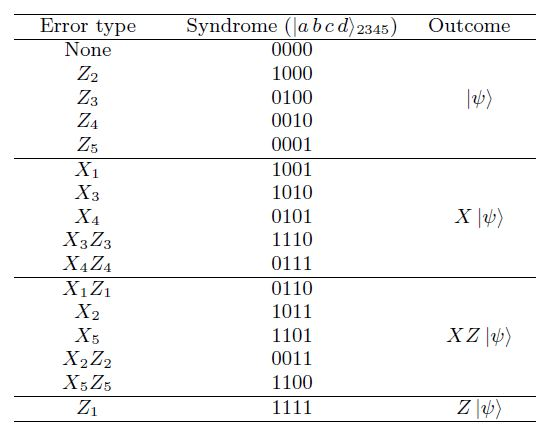
\includegraphics[scale=0.75]{gfx/error_table.JPG}
\caption{Error correction table based on outcomes in auxiliary qubits \citep{joo_error-correcting_2009}}
\label{fig:m_table}
\end{figure}

This process is also represented with a corresponding circuit model in Joo's paper \citep{joo_error-correcting_2009}, included here in figure \ref{fig:m_circuit} to facilitate understanding of the table.

\begin{figure}
\centering
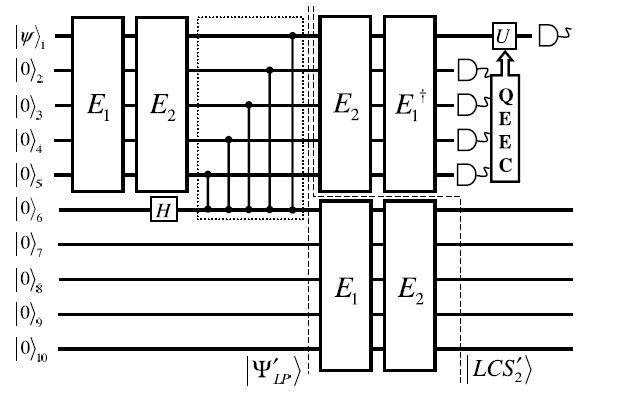
\includegraphics[scale=0.75]{gfx/error_circuit.JPG}
\caption{Full error correction circuit \citep{joo_error-correcting_2009}}
\label{fig:m_circuit}
\end{figure}

%----------------------------------------------------------------------------------------

\section{Higher Complexities}

One of the advantages of this error correction scheme is that it can be easily scaled for the encoding of higher numbers of qubits in each logical state. The conversion for this is simply to scale all operators that act on all three qubits to operate on the number of qubits in the new logical state. The effect of this should be a higher degree of fault tolerance when the error correction scheme is applied.

 % Chapter 3
%% Chapter X

\chapter{Implementation} % Chapter title

\label{ch:implement} % For referencing the chapter elsewhere, use \autoref{ch:name} 

%----------------------------------------------------------------------------------------

\section{Optical Lattices}

Content

%------------------------------------------------

\subsection{Error rates}

Content

%------------------------------------------------

\section{Photons}

Content

%------------------------------------------------

\subsection{Error rates}

Content % Chapter 4
% Chapter X

\chapter{Simulation of One Way Quantum Computation} % Chapter title

\label{ch:simul} % For referencing the chapter elsewhere, use \autoref{ch:name} 

For the next part of the project, a simulation was to be created that would allow for investigation of levels of fault tolerance for different logical qubits in the error correction scheme through Monte Carlo methods. The program would provide simulations of the single gate operations with randomised errors being introduced to the state vector of the system between the encoding and measurement steps. With these randomised errors and by comparing the outputs of the program with expected results, the fault tolerance of each set-up could be determined through repeated running of the program and collection of data. By then comparing the fault tolerance between various sizes of logical qubit in 'triangle' or 'pentagon' states etc, a correlation between fault tolerance and logical qubit size could be established to aid in choice of error correction scheme based on physical parameters of a system.


%----------------------------------------------------------------------------------------

\section{Set-up}

The first step of any simulation is, of course, to establish how the problem will be solved. In this regard, the simulation was first planned in pseudo code and the relevant components sketched out. This plan was somewhat ambitious as it encompassed a scheme for universal applications of one way quantum computation with the described error correction scheme. Though much of this plan was not completed, its contents are described in this section.

%------------------------------------------------

\subsection{Resources used}

For the simulation fortran 95 was chosen as an appropriate language due to it's scalability and ability to be broken up into modules. Details of the compilers, libraries and system used for simulation will be included in Appendix \ref{app:resources}.

Fortran 95 also contained standard functions to call for random numbers that were required for both measurement results and the addition of random errors as well as the ability to determine array sizes intrinsically, allowing for a tidier coding of subroutines.

%------------------------------------------------

\subsection{Subroutines}

A key requirement for the structure of any program was that it would be comprised of subroutines that handled the various steps of the operation of the modelled computer such that these subroutines could be easily rearranged in the main program to simulate any required topological structure. For example, the various single qubit operations required to satisfy universal computation in \citep{raussendorf_measurement-based_2003} can be simulated using the same physical system of a short chain of qubits but with different eigenbases for measurements. Hence in the simulation of a chain of spins the program was designed such that the required measurement operations could be read from a file allowing for any single qubit gate to be simulated with the same program.

Additionally, the two qubit CZ operation was written such that it could be performed between any two qubits in the state vector of the system, allowing it to be used in more complicated programs that would simulate the systems from the triangle states required for the basic implementation of the error correction code to the 8-qubit controlled phase gates.

As such every initialisation and measurement operation was set up to be self contained into one of three modules. The CZ operation module, the measurement module and an additional module that contained several linear algebra procedures required for the program to function. The modular structure also allowed for dynamic array allocation to occur at the top level of the program as array sizes could be passed to the various modules without need to include array sizes as extra arguments in calls to subroutines. This meant that all calls to internal subroutines were reasonably understandable and concise in the coding.

%------------------------------------------------

\subsection{Libraries}

As this program was primarily structured around matrices and linear algebra, extensive use of the BLAS external library as well as the LAPACK library \citep{lapack}. Not only would this make some calculation easier to code, but also meant that the program had some capacity for scalability onto parallel architectures given the structure of the routines in the library. Whenever possible BLAS was used in addition to intrinsic Fortran calls for dot products or matrix multiplication with preprocessor statements allowing the option of compiling without external libraries. However, as the program developed it became more dependant on these libraries and so is no longer functional without them.

%------------------------------------------------

\subsection{Precision}

As the program relied on numerical solutions to systems of linear equations, precision in variables was tantamount to functionality. As such IEEE 754 double precision \cite{_ieee_2008} was used in the program as standard in all real and complex variables, arrays and conversion functions. Because of this machine error was extremely low for all runs of the program, manifesting itself only in null values. While these null values may look untidy in current outputs for the program, they current provide a reasonable guarantee of numerical accuracy and can be easily cleared up in later versions through a rounding step before writing to file. 

However, this would mean that each double precision value in the state vectors of the subroutine or in operation matrices would be using 64 bits for each value stored. Hence the size of the system would quickly cause the memory usage to expand drastically. For a one dimensional chain of qubits, this is not a problem as qubits can be removed from the state vector after measurement, resulting in maximum memory usages of $~128 \times 2^{2}$ for the state vector. In the case of simulation of the quantum Fourier transform described in \citep{raussendorf_measurement-based_2003}, at least 20 qubits would be required, causing memory requirements of $~128 \times 2^{20}$ bits, which would be around 17 megabytes. While this is easily manageable for single qubits, incorporation of the triangle states as an error correction code would require around 18,000 petabytes, a value clearly infeasible for computation as even the top supercomputers have access to even one petabyte \citep{_top500_????} TOP 500 super computers. 

%----------------------------------------------------------------------------------------

\section{CZ Operation}

The first building block subroutine implemented into the program was a CZ operation subroutine. This subroutine would take a state vector and apply a CZ operation based on integer values of control and target bits. In this way, CZ operations could be achieved between any two qubits in the state vector, satisfying the requirements for initialisation of both measurement based single qubit gates and triangle states for error correction.

%------------------------------------------------

\subsection{Kronecker Product routine}

In order to generate the matrix describing the CZ operation between two qubits in the state vector, a subroutine was adapted from previous work \citep{children_spin_2013}, which was updated for Fortran 95's ability to intrinsically determine the size of an array. This subroutine for a Kronecker product was necessary to code as an equivalent was not found in the common external Fortran libraries. 

Using this subroutine CZ matrices were generated from $2 \times 2$ identity and Pauli-z matrices based on the the unitary operator \eqref{eq:u_final3}. 


\insertcode{"code_snippet/Code/cz_gen.f95"}{CZ generation main algorithm}

%------------------------------------------------

\subsection{Improvements}
As the CZ operation matrix is always diagonal, the subroutine could be easily improved to calculate and store the operation matrix as a one dimensional array. This would allow the use of a simpler Kronecker product routine designed only for vectors, but could also make calls to other subroutines unnecessary as the calculation of the operator would be reasonably trivial with a standard formula for generation that required only multiplication of negative numbers into the operator at the appropriate places.

Additionally, the array could be downscaled to integer values and then converted to double precision only when directly applied to the state vector, making savings in computation time and memory usage.

It would also be possible to generate CZ operators for the formation of triangle states similar to the unitary operator in \eqref{eq:logical3plus_u}. By generating these through a separate routine, the application of triangular CZ states shown in the equation \eqref{eq:add_triangle_cz} for the encoding of the logical cluster state, would be optimized further. This operation could even be generalised to satisfy pentagonal, heptagonal or any other alternative formation of logical qubits in the error correction scheme.

%----------------------------------------------------------------------------------------

\section{Other qubit operations}

One requirement for the modules of the program was that circuit model style operations would need to be performed in order to encode the error correction scheme into the system. 

%------------------------------------------------

\subsection{Pauli Z Operation}

While a Pauli Z operation was not coded into the program for single qubits, such a routine would be reasonably simple to implement using a simple modification of the CZ operation subroutine. Fundamentally the CZ operation includes two single qubit Z operations so by removing one of the nested loops the desired effect could be achieved. This subroutine could also be optimised as a diagonal matrix or as integer values in a similar way to the CZ operation, minimising memory usage and computational time.

%------------------------------------------------

\subsection{Hadamard Operation}

Similarly to the Pauli Z operation, the error correction scheme relies on the application of multiple Hadamard operations. Unlike the Z operation, this operator can be required to be applied to multiple qubits at the same time and as such requires a more complicated subroutine. Using the same Kronecker product subroutine it would be possible to form an operator that acts on an array of integers representing qubits to be operated upon. This way any possible error protection configuration could easily be handled by the same subroutine.

While this subroutine could not be held as a single dimensional array like the CZ and Z operations, it could still be stored as an integer, provided a real value be held as an additional variable to reflect the constant value multiplied by the matrix.

%------------------------------------------------

\subsection{Logical Operations}

In order to properly simulate the error correction protocols, the logical operators that are applied for both encoding and error correction need to be incorporated. These operators would be easily handled in the same way as the other operators described earlier as they can be seen to be components of the logical operators. As a result, the logical operator subroutines would operate at a higher level in the program, making use of the basic operators as resources. 

The key condition in designing a subroutine to function such that it can be used for larger logical qubits in order to compare the fault tolerance correlation between logical qubit sizes. This would be trivial to code however as it would just require the number of loops used to apply operations to all of the qubits comprising the logical qubits to be set in the argument of the subroutine rather than hard coded into the program. 


%----------------------------------------------------------------------------------------

\section{Measurement}

Obviously the most vital subroutine for the simulation of the operation of a measurement based quantum computation scheme is the act of measurement itself. Fundamentally, this subroutine must handle the functionality of any quantum algorithms whilst also supporting certain metaphysical principles and assumptions \citep{hagar_quantum_2011}. The program was designed to reflect the same metaphysical assumptions used in the algebraic model earlier and hence the model for measurement used earlier was also applied in the program.

%------------------------------------------------

\subsection{Random measurement in basis}

To reflect the random nature of measurement outcomes in each basis, the intrinsic random number generator in Fortran 95 was employed. This provided a random double precision number between 0 and 1 which was then rounded to the nearest integer value with the intrinsic function NINT(). This provided a simple way to deal with random measurement outcomes whilst also allowing for fixed outcomes in debugging as the default seed for the random number function is consistent, providing identical outcomes on each calling. Whilst seed generation for proper running of the program was explored, the time limited nature of programming meant that such features were never incorporated into the program at large, but it is likely that a seed generation library from the operating system would have been used or a custom one created based on system time.

The integer values representing the outcomes of the measurements were then written to file where they could be retrieved by the subroutine handling the feed-forward of measurement outcomes at the end of the program. 

%------------------------------------------------

\subsection{Pauli bases measurement}

In order to easily model CNOT, Hadamard and $\pi/2$ phase gates, a subroutine for measurement in the three Pauli bases which correspond to the eigenvectors of the $2 \times 2$ Pauli matrices was incorporated into the program. As these measurement bases were commonly used in almost all qubit gates it made sense to have them hard coded into the program instead of using a single generalised measurement routine 

\begin{equation}
\begin{array}{lclc}
  \sigma_{x+}=\displaystyle\frac{1}{\sqrt{2}}\!\!\!\!\! & \begin{pmatrix}{1}\\{1}\end{pmatrix}, & \sigma_{x-}=\displaystyle\frac{1}{\sqrt{2}}\!\!\!\!\! & \begin{pmatrix}{1}\\{-1}\end{pmatrix}, \\
  \sigma_{y+}=\displaystyle\frac{1}{\sqrt{2}}\!\!\!\!\! & \begin{pmatrix}{1}\\{i}\end{pmatrix}, & \sigma_{y-}=\displaystyle\frac{1}{\sqrt{2}}\!\!\!\!\! & \begin{pmatrix}{1}\\{-i}\end{pmatrix}, \\
  \sigma_{z+}=                                          & \begin{pmatrix}{1}\\{0}\end{pmatrix}, & \sigma_{z-}=                                          & \begin{pmatrix}{0}\\{1}\end{pmatrix}.
\end{array}
\end{equation}

In order to keep the programming concise, all three kinds of basis were included into the same subroutine which was controlled by a single character in the argument of the subroutine. This character would then be recorded in a file containing data about the measurements that could be used to calculate the final states in the feed forward subroutine. Currently however the program uses the phase directly, but this could be optimised in future iterations by hard coding the phase amounts of the Pauli bases into the feed forward routine. Unfortunately the Pauli Y and Pauli Z basis measurements do not work in the program when it comes to the final feed forward of measurement because of an error with the phase of the basis when it comes to feed forward of measurements to obtain the final state, so this change might even help alleviate that problem.

%------------------------------------------------

\subsection{Arbitrary measurement}

In addition the the Pauli bases measurements, a generalised measurement of arbitrary phase was also required for the program to implement the general rotation and z rotation single qubit gates. The subroutine for this process was very similar to the Pauli measurement subroutine aside from the inclusion of a variable measurement phase in the arguments of the subroutine and a general rotation vector replacing the eigenvectors of the Pauli bases. 

The subroutine, like the Pauli measurement subroutine, recorded the variable phase amount to a file so that it could be used in the feed forward subroutine as well as multiplying the result of the inner product of the measurement vector and the measured qubit state vector by the global state vector. Potentially this subroutine could be consolidated into the Pauli measurement subroutine through the use of the control character, likely with 'R' signifying a custom phase, but this is yet to be performed.

%------------------------------------------------

\subsection{Feed Forward}

The final necessary component of the measurement scheme consisted of a subroutine to feed forward measurement outcomes to recover the desired state at the end of the measurements. This subroutine performed the functionality of equation \eqref{eq:one_qbit_feed_forward} for the single qubit states. 

In order to achieve this result, the subroutine read the measurements performed over the course of the program in order and then applied \eqref{eq:one_qbit_feed_forward} for each measurement, leading to accurate results. 

The subroutine also has the functionality of being able to decompose larger state vectors in order to apply the feed forward results to specific qubits, but this is feature is currently unfinished.

%------------------------------------------------

\subsection{Multiple Outputs}

One of the weaknesses of the current subroutine to handle the feed forward of measurements is that it cannot deal with output state vectors consisting of multiple qubits simultaneously. For example, in the output state of the CNOT gate in equation \eqref{eq:CNOT_qbit_feed_forward}, a series of decoding operations are required to be performed on two qubits at once, which the subroutine would not be able to handle. 

Fortunately this is only a minor problem as the error correction scheme only requires a single output qubit and with sufficient time the subroutine could be updated to deal with such problems if deemed necessary.

%----------------------------------------------------------------------------------------

\section{Decomposition}

One of the critical elements to the functionality of the program was the ability to decompose the global state vector into individual qubit states in order for both the simulated measurement to be processed and the final state of the qubit to be determined. This required a reversing of the Kronecker product routine used to generate the state vector which presented a formidable challenge computationally.

While Kronecker products are not directly reversible, it is possible to determine a 'canonical' result for certain matrices. The principle behind this relies upon the relation between the Kronecker product and the vectorisation operator. Considering the vector $W$ which is a Kronecker product of two real vectors $U$ and $V$:

\begin{equation}
W = V \otimes U = vec(U V^{T})
\end{equation}

Vectorisation is a process which is easily reversed, so the vectors U and V can be recovered by decomposition of the resulting matrix. Note that for complex vectors $V^{T}$ becomes $V^{H}$ which represents the conjugate transpose of $V$.

\begin{equation}
U V^{T} = vec^{-1} (W)
\end{equation} 

Unfortunately, there are a wide range of possible decompositions, so this is where a canonical decomposition must be decided upon in order to progress further. 

%------------------------------------------------

\subsection{Rank decomposition}

The first subroutine developed to perform this decomposition was a simple rank 1 decomposition. It was originally thought that this would be sufficient in all cases as the Kronecker product of two vectors would always be rank one. However this was short-sighted as the application of the CZ operation modified the rank of the state vector, a phenomenon which seems to be representative of the entanglement induced in the system.

The algorithm worked by pulling the first non-zero column of the matrix formed from the inverse vectorisation of $W$ and normalising it. Then the algorithm divided each value of the first non-zero row by the new normalised values to obtain the other vector.

For a rank 1 state vector of pure such as $\ket{00}$ the algorithm was successful, but when encountering mixed states, the algorithm could not handle the input and returned null values. This was obviously unacceptable as the CZ operation will always make mixed states out of pure input states.

\insertcode{"code_snippet/Code/r1_decomp.f95"}{Rank decomposition algorithm}

%------------------------------------------------

\subsection{Single value decomposition}

As the rank decomposition was not a sufficient way to canonically decompose the matrix, the single value decomposition (SVD) was chosen as an alternative. As this was an $M \times N$ decomposition it would allow for particular qubits to be determined, compared to something like the eigen-decomposition which would only work with square matrices and thus be only able to break the state vector in half. 

Fortunately, unlike the rank decomposition there are plenty of available libraries for single value decomposition. For the simulation the double precision complex general decomposition routine zgesvd was chosen from the LAPACK library as it both complied with the established IEEE 754 precision standard and allowed for decomposition of a general matrix.

However, the SVD is a little more complicated than the rank decomposition as the matrix is broken into three parts. In the case of a complex matrix these consist of a diagonal matrix $\boldsymbol{\Sigma}$ of the singular values $\sigma_{i}$ of the matrix and two matrices $\mathbf{U}$ and $\mathbf{V}$ composed of rows and columns of vectors such that:

\begin{equation}
\mathbf{M} = \mathbf{U} \boldsymbol{\Sigma} \mathbf{V}^{H}
\end{equation}

When performing this decomposition in the program the resulting vectors $U$ and $V^{H}$ were assumed to be the summations of the rows or columns of matrices $\mathbf{U}$ and $\mathbf{V}$ respectively, while the $i$-th rows of $\mathbf{U}$ were multiplied by the corresponding single values $\sigma_{i}$.

The routine was tested with the application of a pauli X basis measurement on a pair of two qubits initialised in the $\ket{+}$ state before having the CZ operation applied. The resulting state vector of this initialisation was:

\begin{equation}
W =
\begin{pmatrix}
\frac{1}{2} \\
\frac{1}{2} \\
\frac{1}{2} \\
- \frac{1}{2} \\
\end{pmatrix}
\end{equation}

So when inverse vectorisation was applied this became:

\begin{equation}
\mathbf{M} =
\begin{pmatrix}
\frac{1}{2} &
\frac{1}{2} \\
\frac{1}{2} &
- \frac{1}{2} \\
\end{pmatrix}
\end{equation}

When entered into the subroutine the output was:

\begin{align}
\mathbf{U} &=
\begin{pmatrix}
-\frac{1}{\sqrt{2}} &
-\frac{1}{\sqrt{2}} \\
-\frac{1}{\sqrt{2}} &
\frac{1}{\sqrt{2}} \\
\end{pmatrix}
&
\boldsymbol{\Sigma} &=
\begin{pmatrix}
\frac{1}{\sqrt{2}} &
0 \\
0 &
\frac{1}{\sqrt{2}} \\
\end{pmatrix}
&
\mathbf{V}^{H} &=
\begin{pmatrix}
-1 &
0 \\
0 &
-1 \\
\end{pmatrix}
\end{align}

So the vectors $U$ and $V$ became:

\begin{align}
U =
\begin{pmatrix}
\frac{2}{\sqrt{2}} \\
0 \\
\end{pmatrix}
V =
\begin{pmatrix}
\frac{1}{\sqrt{2}} \\
\frac{1}{\sqrt{2}} \\
\end{pmatrix}
\end{align}

When the measurement in the Pauli X basis was applied, in case one:

\begin{multline}
\ket{+} \braket{+|U} \otimes \ket{V} \\
= \ket{+} (\frac{1}{\sqrt{2}}\frac{2}{\sqrt{2}} \braket{0|0}) \otimes \ket{V} \\
= \ket{+} \otimes \ket{V} \\
\end{multline}

Feeding the measurement result forward to determine the output state then gives:

\begin{equation}
e^{0} X^{0} H R_{0} \ket{V}
= H
\begin{pmatrix}
\frac{1}{\sqrt{2}} \\
\frac{1}{\sqrt{2}} \\
\end{pmatrix}
= \ket{0}
\end{equation}

Similarly for the other measurement outcome:

\begin{equation}
e^{0} X^{1} H R_{0} \ket{V}
=  X H
\begin{pmatrix}
\frac{1}{\sqrt{2}} \\
\frac{1}{\sqrt{2}} \\
\end{pmatrix}
= \ket{1}
\end{equation}

These outcomes match the expected outcomes for measurements of the qubit in the pauli X basis which is easily seen by looking measurement of the state expressed in the form described in equation \eqref{eq:2qubit_example}. In case 1:

\begin{equation}
\label{eq:m_outcome_1}
\bra{+} \frac{1}{\sqrt{2}} (\ket{+ 0} + \ket{- 1}) = \ket{0} = H \ket{+}
\end{equation}

And in case 2:

\begin{equation}
\label{eq:m_outcome_2}
\bra{-} \frac{1}{\sqrt{2}} (\ket{+ 0} + \ket{- 1}) = \ket{1} = XH \ket{+}
\end{equation}

Unfortunately the decomposition has not been tested for larger or more complex state vectors due to time constraints. However, it seems like there will be certain matrices which will throw up errors due to the multiplication of zero values or through the summation of rows and columns being zero, this could be fixed by performing multiple decompositions until a satisfactory decomposition for which zero values are minimised is achieved, but this would take extra computational resources and be mathematically untidy. In this regard, it seems that there must be a better way to reconstruct the vectors from the decomposition matrices but so far this remains unclear.


%----------------------------------------------------------------------------------------

\section{Error}

One of the crucial functionalities a completed program would be the ability to add randomised errors to a single or multiple qubits in a state vector of any size in order for the fault tolerance of each system to be analysed. Such a subroutine was only in its early stages in the program as it had not yet advanced to the stage of implementation of the error correction scheme necessary for the subroutine to be meaningful, but a clear plan had been drawn up as to how errors would be implemented numerically into the system. Ideally error would be induced between the CZ and measurement operations, as this would be consistent with the state vector that is resilient to errors in the error correction scheme, but error could be easily added to the state vector of the system at any time.

%------------------------------------------------

\subsection{Flip error}

Flip errors are reasonably easy to simulate in the state vector in any size as they can be effectively expressed as the application of a Pauli X operation to a qubit. In order to operate on a single qubit, or multiple, the Kronecker product subroutine would be employed to form operator matrices of appropriate size in a similar fashion to the way operators would be used to initialise the system with the error correction scheme. For example the operator operation applied to flip qubit $i$ in a state vector of $N$ qubits would be:

\begin{equation}
\mathbb{1}_{1} \otimes \mathbb{1}_{2} \otimes \dotsb \sigma_{X} \dotsb \otimes \mathbb{1}_{N}
\end{equation}

It is therefore clear that such an operator could easily be produced with nested loops of the Kronecker product subroutine, what remains unclear however is as which qubits the flips would be applied and at what rate. 

The simple way to decide which qubits to flip would be to have a universal error rate for bit flips and then include either Pauli operators or identity operators depending on whether a random number meets the threshold of the error rate. This would have the bonus effect of saving memory and calculation time compared to performing each flip individually as well as simplifying the programming of any subroutine handling errors.

The alternative to this would be to have separate error rates for each number of errors so that the number of errors are calculated and then assigned to random qubits in the following step. This would be particularly useful when testing whether the error correction scheme protects against particular numbers of phase flips, though would obviously cause a slight interest in computational requirements.

One advantage to only modelling phase flips however is that any operator matrix can be stored in integer form and only converted to double precision when multiplying out with the state vector. This would save large amounts of memory compared to a phase error matrix which would require double precision storage and thus have memory requirements equal to the square of the memory requirements of the state vector.

%------------------------------------------------

\subsection{Phase error}

Similarly to the flip error, phase errors can be simulated through the inclusion of a phase operation on a qubit in the state vector. However, the phase of the error present provides another variable for the model as phase errors are obviously continuous variables rather than the discrete flip errors. Hence not only would a random number of qubits need to be exposed to the error, the exact value of the error would also need to be determined. While this could be done with a fixed error, something like a Gaussian distribution would work reasonably well for modelling. Indeed, if a a Gaussian distribution with a particularly high standard deviation were used, Phase errors could be applied to every qubit, reducing the number of steps in calculation of the operator. 

%----------------------------------------------------------------------------------------

\section{Data Analysis}

Another key component for the program is the ability to analyse cohesive and accurate output data. This puts requirements on the format of output data as well as the method of storage. For the program in its current form, data is output formally from the fidelity function, the value of the state vectors is printed directly to standard output, which was typically piped into a separate file.

%------------------------------------------------

\subsection{Fidelity}

In order to determine if the output state and expected output state correspond to one another, a fidelity subroutine was also included in the program. Like the Kronecker product subroutine, this subroutine was adapted from earlier work and simply performed the basic calculation:

\begin{equation}
\text{Fidelity} = |\braket{\text{Expected State}|\text{Final State}}|^{2}
\end{equation}

Like the other subroutines in the program, this calculation could be performed with or without the BLAS library's complex double precision dot product routine (ZDOTU) and as such has potential for scalability into parallel processing.

%------------------------------------------------

\subsection{Bulk data}

The ideal end result for a complete program would involve a large data set of fidelity data from multiple runs of the program. As a result some changes would have to be made so that fidelity data was instead appended to the file. Once this had been done, a scatter plot between the number of gates performed on the data and the fidelity of the result would be plotted for each size of logical qubit. 

This data would then be fitted to a curve using whatever method best worked for the output in order to establish the correlation between the two axes depending on the fixed error rate from the program. This would hopefully lead to a better understanding of the way in which fault tolerance was affected by the size of logical qubits for this measurement scheme.

%----------------------------------------------------------------------------------------

\section{Error Correction Scheme}

The final part of the program is the incorporation of the error correction scheme. This involves two main subroutines, the encoding subroutine and the detection/correction subroutine. 

%------------------------------------------------

\subsection{Encoding}

The encoding subroutines main function would be reflective rotational operation combined with the method for forming logical CZ operators described in section \ref{sec:entag_3_qb}. This would be challenging to perform and would require a great deal of coding in order for the operations to be scalable to any size logical qubit.

%------------------------------------------------

\subsection{Correction}

Correction, in comparison, would be a little easier to implement as the measurement routine currently in use for the program could be recycled for the bulk of the functionality. The main challenge would then be the conditional statements to implement the scheme and apply the appropriate logical operations depending upon the measurement outcomes. There would also need to be a small decoding step also, but this could be adapted from the encoding step which would need to be implemented first for correction to be possible in the first place.

%----------------------------------------------------------------------------------------

\section{Other structures}

In addition to testing the error correction scheme on single qubit gates, there are some other gates and set-ups that would be both interesting and useful to simulate with the program. These structures are of interest in particular as they represent the key building blocks of common quantum algorithms.

%------------------------------------------------
\subsection{Controlled not gate}

The first interesting structure that would make a good extension to the program would be a controlled not gate, though implementation would require the problems with the feed forward subroutine being unable to deal with multiple qubit state vectors to be rectified.

Obviously one of the advantages of demonstrating that this structure can be fault tolerant is that, when combined with the single qubit gates, forms a universal set of quantum gates. This means that such a demonstration would be necessary to prove the validity of the error correction scheme as universal.

Unlike the single qubit gates, it would not be possible to perform this operation repetitively without the introduction of new control qubits. While this is not too difficult a problem to overcome, it would make comparison of final results with expected outcomes more challenging as the expected outcomes would require far more calculation than repetitive use of a $\pi / 2$ gate, for example.

%------------------------------------------------

\subsection{Controlled phase gate}

A very interesting structure for simulation by the program, would be a controlled phase gate. This structure is interesting both because not only can it be represented without the decompositions into CNOTs and rotations required for the circuit model, but it is also a crucial building block for the Quantum Fourier transform algorithm \citep{raussendorf_measurement-based_2003}. 

\begin{figure}
\centering
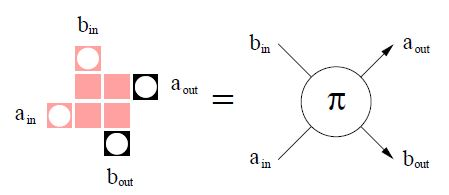
\includegraphics[scale=0.9]{gfx/phasegate.JPG}
\caption{Controlled phase gate structure and functionality
 \citep{raussendorf_measurement-based_2003}}
\label{fig:phase_gate}
\end{figure}

This structure, show in figure \ref{fig:phase_gate}, consists of 8 qubits in a spiral pattern with measurements performed on the central square, far simpler than the chain of gates required in the circuit model. However, like the CNOT gate, implementation of a measurement feed forward subroutine that could handle multiple outputs would be required. Implementation of this structure into the model with the error correction code would be also quite interesting given the entanglement of four qubits simultaneously, which would present an interesting programming challenge.

%------------------------------------------------

\subsection{Quantum Fourier transform}

If the program can simulate controlled phase gate, the Fourier transform is also possible with sufficient computational resources. As shown in 'Measurement-based quantum computation on cluster states', this structure can be constructed from six controlled phase gates and three Hadamard gates \citep{raussendorf_measurement-based_2003}. This particular structure is of great interest as it forms a crucial part of Shor's algorithm, making implementation highly desirable. However, memory usage of implementation for this structure in conjunction with an error correction scheme would be problematic given its high requirements on the number of qubits that are simultaneously active. It is possible that the components of the structure could be broken down in order to minimise the required computational resources through the inclusion of unitary gates between controlled phase gates and the simulation of each phase gate individually, but as yet this seems difficult to envision.

\begin{figure}
\centering
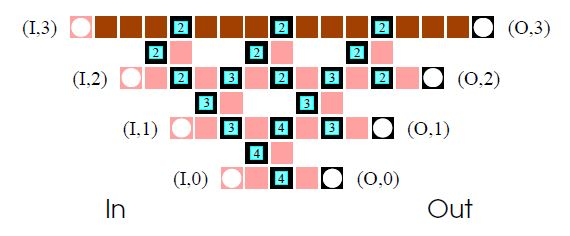
\includegraphics[scale=0.75]{gfx/qft.JPG}
\caption{Quantum Fourier transform schema \citep{raussendorf_measurement-based_2003}}
\end{figure} % Chapter 5
%% Chapter X

\chapter{Simulation of Logical States} % Chapter title

\label{ch:sim_log} % For referencing the chapter elsewhere, use \autoref{ch:name} 

%----------------------------------------------------------------------------------------

\section{Set-up}

Content

%------------------------------------------------

\section{Error}

Content

%------------------------------------------------

\section{Analysis}

Content % Chapter 6
% Chapter X

\chapter{Conclusions} % Chapter title

\label{ch:conclu} % For referencing the chapter elsewhere, use \autoref{ch:name} 

Due to the very unfinished nature of the program, few conclusions can be drawn about the fault tolerance of the error correction scheme, however things can be learned from the challenges encountered while programming so that such problems can be averted in later versions of the program as well as in other programming based projects.


%----------------------------------------------------------------------------------------

\section{Choice of resources}

It was found that Fortran is very much an appropriate language of choice for this kind of program given its access to a wide range of linear algebra libraries and the ease of constructing modular programs. If the program were to be adapted for parallel processing, this language would continue to work well give its access to these libraries, likely in conjunction with openMPI. Otherwise, it might be better if it were converted to python due to python's better handling of complex numbers and the removal of the need to compile the program, something which would be of benefit while many values in the program are still hard coded. 

%----------------------------------------------------------------------------------------

\section{Matrix Decomposition}

As a way of recovering the individual state vectors of particular qubits from the larger state of the system, matrix decomposition is incredibly unreliable. While this can be mitigated to a certain extent by intelligent use of algorithms that form canonical decompositions such as the single value decomposition or eigen-decomposition, there are likely to always be problems with certain values as the complexity of superposition for the state vector increases. Fortunately this is not too large a problem for they systems in this project as they would rarely exceed six qubits or so, but it seems like a big issue for larger systems. 

It seems possible that rather than just being a mathematical challenge, the difficulty in decomposing a matrix to accurately represent individual state vectors is more of problem resulting from the foundations of quantum mechanics. The difficulty in taking apart a state vector for mixed states is a mathematical reflection of the tricky nature of superposition and is unlikely to ever be resolved easily.


%----------------------------------------------------------------------------------------

\section{Further Work}

While this work is unfinished, it also has a lot of potential for extension, this includes both the planned features that were not included to the program and the inclusion of the more complex structures that have interesting implications. As a result the work for this project will be continued independently of the end of the course in order to resolve the outstanding questions. 

If the program can be rebuilt into a more concise package with better modules, it may even serve as a useful tool for students interested in one way quantum computation as it provides a clear outline of the process in several easy to understand modules.  % Chapter 7
% Chapter X

\chapter{Additional Work} % Chapter title

\label{ch:additional} % For referencing the chapter elsewhere, use \autoref{ch:name} 

With the failure of the program to simulate any measurement other than Pauli X basis measurements, further work was required in order to properly develop the program into a fully functional simulation of one way quantum computation before moving onto simulation of error correction schemes. he primary criteria was therefore to develop a simulation of the four single qubit gates required for universal computation. This was attempted through debugging of the program as well as numerous improvements to its functionality, which are described in the following sections.

%----------------------------------------------------------------------------------------

\section{Errata}

A number of mistakes were made in the earlier body of work, this section describes the corrections made to the simulation to rectify those problems. 

%------------------------------------------------

\subsection{Basis measurement}

One major issue for the program was that the value for the Z Pauli eigen-basis measurement vector was incorrectly entered as to be identical to that of the X Pauli eigen-basis measurement in the Pauli basis measurement subroutine. This was a minor issue as the Z basis measurement functionality was unused as only single qubit gate operations were ever being simulated simultaneously so that the Z measurement was not required in order for qubits to be removed from the cluster. Despite this, because of the nature of the Z basis measurement as a disentangling operation, in order for it to be used in the simulations modifications to the feed forward operations would need to be implemented to accommodate the effect of Z measurements on the output states in the program. These operations would be required when simulating multi qubit gates if the system was initiated as a 2D lattice instead of directly as the cluster state for the gate. This would be necessary for further iterations of the program. One way to deal with this however would be simply to assume that all Z measurement outcomes are $m_{i} \in \set{0}$ just as in \textit{"Measurement-based quantum computation on cluster states"} \citep{raussendorf_measurement-based_2003}. Doing this would negate the need for Z operations to be fed forward as they would not effect the output state of the simulation if this condition was met.

%------------------------------------------------

\subsection{Normalisation}
\label{subsec:normal}
One issue that was presenting itself for longer chains of qubits was the lack of normalisation after measurement. This meant that the output information states were acquiring a factor of $1 / \sqrt{2}$ after each measurement due to the factors introduced by the CZ operation not being completely removed. In earlier versions this was not apparent due to other errors in the measurement simulation algorithm that counterbalanced the effect, giving Pauli X basis measurements that seemed correct despite being a factor of $\sqrt{2}$ too large. 

The effect of this was missed during the theoretical work for equations \ref{eq:m_outcome_1} and \ref{eq:m_outcome_2}, where a factor of $1 / \sqrt{2}$ mysteriously disappears between the left and right side of the equation. Once other errors in the algorithm were corrected, upon multiple iterations of the program the magnitude of the vectors was being increasingly small, which was concerning until this flaw was identified through debugging.  

\begin{equation}
\bra{+} \frac{1}{\sqrt{2}} (\ket{+ 0} + \ket{- 1}) = \ket{0} = H \ket{+}
\tag{\ref{eq:m_outcome_1}}
\end{equation}

\begin{equation}
\bra{-} \frac{1}{\sqrt{2}} (\ket{+ 0} + \ket{- 1}) = \ket{1} = XH \ket{+}
\tag{\ref{eq:m_outcome_2}}
\end{equation}

By normalising after the steps from these two equations, this factor is negated and this was done by including this normalisation into the algorithm used for measurement as described in subsection \ref{subsec:normal}.

%------------------------------------------------

\subsection{Feed forward operators}

In the subroutine dealing that handled output of the correct output states from the simulation, the operators were applied in the incorrect order as they were mistakenly chosen to be the operators that are applied to the information state as a result of measurement from equation \ref{eq:one_qbit_feed_forward}, the complete opposite of the intended effect.

\begin{equation}
\ket{out^{m_{i}}}_{2} = e^{\frac{-i \psi}{2}} X^{m_{i}} H R_{z} (-\phi) (a \ket{0}_{2} + b \ket{1}_{2})
\tag{\ref{eq:one_qbit_feed_forward}}
\end{equation}

However the operators were being applied such that:

\begin{equation}
\ket{\psi} = e^{\frac{-i \psi}{2}} X^{m_{i}} H R_{z} (-\phi) \ket{out^{m_{i}}}_{2}
\end{equation}

The inverses of these operators should have been applied to recover the output of computation such that:

\begin{multline}
\ket{\psi} = (e^{\frac{-i \psi}{2}} X^{m_{i}} H R_{z} (-\phi))^{-1} \ket{out^{m_{i}}}_{2} \\
= e^{\frac{-i \psi}{2}} R_{z}^{-1} (-\psi) H X^{m_{i}}\ket{out^{m_{i}}}_{2} \\
\end{multline}

This explains part of the reason as to why the X basis measurement was working while Y basis and arbitrary measurements on the X-Y plane were not as the inverse of this group of operators is equal to itself when $\phi = 0$ and the measurement outcome is $0$, as can be the case when Pauli X basis measurements are applied. This is not the case for non zero values of $\phi$ so these values were displaying errors. In newer versions of the simulation, the inverse of the rotation operator is now correctly utilised while the Pauli-X and Hadamard operators remain the same as they are their own inverses.

To accompany this change, the order in which the operators were applied was also changed through modifications to the data formats handled by file I/O detailed in subsection \ref{subsec:data_form}. This was needed because the operators had to be implied in the inverse order of those in the original program. Additionally, to simplify the program the external phase factor was included in the inverse z-axis rotation operator matrix such that:

\begin{equation}
e^{\frac{i \theta}{2}} R_{z}^{-1}(- \theta) = 
\begin{pmatrix}
e^{\frac{- i \theta}{2}} & 0 \\
0 & e^{\frac{i \theta}{2}} \\
\end{pmatrix}
=
\begin{pmatrix}
1 & 0 \\
0 & e^{i \theta} \\
\end{pmatrix}
\end{equation} 

Which is also the single qubit phase gate operator $P_{\theta}$. This means that the feed forward operators applied for $n$ measurements became:

\begin{equation}
\ket{\psi}_{n + 1} = \prod\limits^{n}_{i= 1} 
(P_{\theta}(\phi_{i}) H X^{m_{i}}) \ket{out}_{n + 1}  
\end{equation}

This would also satisfy the condition for by-product operators specified in \textit{"Measurement-based quantum computation on cluster states"} \citep{raussendorf_measurement-based_2003}, which states that by-product operators are composed of Pauli vectors as $P_{\theta}$ becomes $\sigma_{z}$ when $\theta = \pi$.

%------------------------------------------------

\subsection{Measurement subroutine}
\label{subsec:M_subroutine}

One very significant change is the way in which measurement of single qubits are handled by the measurement subroutines. It was determined that one of the central issues of the program arose due to the insufficiency of the algorithm in the handling correct super-positions correctly. This was due to an arbitrary addition of the rows of the $U$ matrix of the single value decomposition to form a vector for computation of inner products as well as an arbitrary addition of the columns of the $V$ matrix as shown in \eqref{eq:bad_math}.

\begin{equation}
\label{eq:bad_math}
\ket{\psi} = \ket{m} \bra{\sum\limits_{j=1}^{n} U_{j}} \sum\limits_{i=1}^{n} S_{i} V_{i}
\end{equation}

While this appeared to provide the correct output state for some measurements, Y basis measurements would be widely inaccurate as the complex component would be multiplied by zero, rendering the measurement ineffective and completely non-physical. This older version of the algorithm is shown in listing \ref{list:old_m}.

\insertcode{"code_snippet/Code/old_measurement.f95"}{Old Measurement Algorithm \label{list:old_m}}

To solve this problem, a modification to the algorithm was devised in order to preserve as much of the structure of the program as possible. The \textit{get\_vector\_complex()} subroutine was changed to also pass the values of the output of the single value decomposition to the measurement subroutine so that they could be used directly on a higher level or layer of the program. This limited the functionality of the \textit{get\_vector\_complex()} subroutine to effectively nil however as it was now only able to pass variables from either the first or the last qubit in the chain.

Next, the output state was changed to be represented by the sum of the inner products between the vector of measurement and each column of of the U matrix from the single value decomposition, which was then multiplied by the single values and the rows of the transpose matrix VT. This new approach is shown in listing \ref{list:new_measurement}. The normalisation after measurement described in section \ref{subsec:normal} can be also seen in listing \ref{list:new_measurement} as the factor of $\sqrt{2}$ multiplying the output state. 

\insertcode{"code_snippet/Code/new_measurement.f95"}{New Measurement Algorithm \label{list:new_measurement}}


This new approach prevented the obvious errors with arbitrary measurements from being produced by the simulation, particularly ones that would become larger in magnitude than 1, values which were invalid for quantum information states. 

%------------------------------------------------

\subsection{Numerical Value Precision}

A minor issue in the program was the fixed parameter for $\pi$ was being incorrectly entered into the program as single precision complex instead of double precision complex. This had the effect of increasing the machine error in the program by a factor of 8, which was fortunately still small. However, this was becoming increasingly manifest when larger chains of qubits were attempted. This was rectified by specifying the number kind on the entry of the value in the header part of the measurement module.

More generally, there are perhaps some issues with the programs outputs for zero values in state vectors and operators output by the program for debugging. As would be expected these values are now equal to the machine error for the complex 16 format, but it may be more useful to reformat them to zero either after an iteration of the program or upon output of values. This would be risky when simulated error in the physical system is added to the program however as the processes dealing with machine error may not be able to distinguish between machine and simulated error. As long as the simulated errors are larger than the machine error by several orders of magnitude this shouldn't be too great a concern as subroutines could be devised to distinguish between them based on this condition.


%----------------------------------------------------------------------------------------

\clearpage
\section{Adjustments and Improvements}

In addition to the correction of errors in the program, numerous improvements to the efficiency and functionality of the program were also made.

%------------------------------------------------

\subsection{Rearrangement of fidelity function}

The first modification made to the program concerned the overall internal logical structure of the program. In order to standardise the arguments of subroutines within the program, the fidelity subroutine was moved into the the measurement module and altered to become a function. This allowed the elimination of the array size operator as had already been performed with the linear algebra routines and the need for an additional variable for fidelity in the main program. While this will not have changed much for the performance of the program due to compilation optimisation, it makes the program more adaptable and facilitates understanding of its workings.


%------------------------------------------------

\subsection{Measurement subroutine}
\label{subsec:m_sub_improv}

In addition to modifications to the fidelity subroutine, much of the measurement subroutines were overhauled. The two subroutines for Pauli basis and general measurement were merged into one whilst the random measurement outcomes were externalised to a separate subroutine that also dealt with the various types of measurement. Additionally the file output was moved to an additional external subroutine to facilitate alternative methods as measurement, such as those utilised later in section \ref{sec:larger_chain}.


This reconfiguration had an added bonus of allowing use of routines externally in program, where it was necessary to call for the types of measurement that the program was instructed to simulate. One example of this would be in the feed forward of measurement operators in for the multiple qubit cluster states where it became necessary to call for information about the measurements in order to determine the correct order to perform operations as well as acquire the appropriate measurement vector so that it could be separated from the larger state vector of the system.

%------------------------------------------------

\subsection{Libraries}

As the program became increasingly dependent upon external subroutines for linear algebra, some functionality previously performed by intrinsic functions was replaced by calls to the BLAS library. Particularly in places where compiling with or without BLAS was dependent on preprocessor control sequences. This meant that those preprocessor directives could simply be removed and the file names modified to prevent automatic preprocessing by the compiler regardless of flags.

%------------------------------------------------

\subsection{Data format}
\label{subsec:data_form}


One of the issues raised by the correction to the order of application of operators in the reversal of the by-product operators by the feed forward subroutine was access to the files containing information about the measurements performed on the system. This was because the file containing measurements now needed to be read in reverse order as the correction for the first by-product operator needed to be applied last. Unfortunately there seemed to be no way to read a file directly in reverse with Fortran's intrinsic I/O, so modifications to the data format were made to include a key for each measurement outcome so that each measurement could be read directly. Now each file is read in the correct order by accessing the record for the keys in reverse order and applying the appropriate operators.

%----------------------------------------------------------------------------------------

\section{Program outputs}

Once again, the outcomes for the program had a host of issues despite the new corrections and improvements. As before, X measurement operations correctly formed a one bit teleportation which could be repeated for any length of chain, but problems arose when other operations were utilised. 

The issue that drew most attention was realisation of the $\frac{\pi}{2}$ gate, which formed a benchmark for the functionality of Y basis measurements. In theory, this gate should be realised for a chain of five qubits through four measurements in the XXYX bases. However, the output of the program was identical to the input regardless of measurement outcomes, presenting a huge problem for the correctness of the simulation. Upon investigation, it was discovered that the gate could be realised correctly if the phase angle in the $P_{\theta}$ operator used to correct for the by-product operators was doubled. When this modification was made, a $\frac{\pi}{2}$ gate was fully realised, but only for measurement outcomes of zero. If the outcome of the four measurements was one the gate would be realised through an additional Z operator.

Similarly, when simulation of the Hadamard gate, through XYYY measurements on an identical system, the final output was identical to that of four X measurements (i.e. the input state had been teleported to the fifth qubit). However, when the phase in the $P_{\theta}$ operator was doubled, the output states would be superposition of the real and complex Hadamard output. For example when $\ket{+}$ was the input, the output was $\frac{i - 1}{2} \ket{0}$. 

Even without correction for by-product operators the output from the simulations were incorrect, meaning that the problems with the simulation must be in the way measurement was being performed, though a thorough investigation into the problem yielded no results. Additionally, when attempting to derive the by-product operators specified in \textit{"Measurement-based quantum computation on cluster states"} \citep{raussendorf_measurement-based_2003}, independently from the generalisation of the by-product operators being utilised the formulations differed leading to the view that the simulation was also insufficient in this regard. For example, when attempting to derive the by-product operator for the $\frac{\pi}{2}$ gate the operator was:

\begin{equation}
U = \sigma_{x}^{m_{4}} H \sigma_{x}^{m_{3}} H R_{\theta}(- \phi) \sigma_{x}^{m_{2}} H \sigma_{x}^{m_{1}} H
\end{equation}

Applying the relation $XH = ZH$ and assuming that either $\phi$ or $R_{\theta}(- \phi)$ is such that $R_{\theta}(- \phi) = Z$.

\begin{multline}
U = \sigma_{x}^{m_{4}} \sigma_{z}^{m_{3}} \sigma_{z} \sigma_{x}^{m_{2}} \sigma_{z}^{m_{1}} \\
= \sigma_{x}^{m_{4} + m_{2}} \sigma_{z}^{m_{3} + m_{1} + 1} \\
\end{multline}

Comparing this to the by-product operator for the $\frac{\pi}{2}$ described in \textit{"Measurement-based quantum computation on cluster states"} \citep{raussendorf_measurement-based_2003}:

\begin{equation}
U_{\Sigma, U_{z} (\pi / 2)} = \sigma_{x}^{m_{4} + m_{2}} \sigma_{z}^{m_{3} + m_{2} + m_{1} + 1} 
\end{equation}

So the formulation of by-product operators in the program does not match the by-product operators in the paper, which would explain why the output state would have been correct, for measurement outcomes of 1, if the if an additional $\sigma_{z}$ operation had been applied. Interestingly enough, just applying a single Y operation on a chain of 2 qubits will realise the $\frac{\pi}{2}$ gate for both possible measurement outcomes. This would seem to indicate that the by-product operators are either incorrectly formulated or specific for the type of gate being realised.  Unfortunately, the by-product operators described in the paper for the Hadamard gate cannot be used to correct for the problems with the Hadamard gate in the same way so it is likely that the problem with the program occurs before the feeding forward of measurement outcomes.


As this problem concerned larger states, it was decided not to proceed onto simulation of the error correction scheme due as it was reliant on clusters of at least four qubits being measured reliably. Instead focus was directed to attempting to solve the problems at hand so that a better understanding of the simulation could be obtained as well as find ways of performing the simulation more efficiently. 

%----------------------------------------------------------------------------------------

\section{Larger chain program}
\label{sec:larger_chain}

As the single qubit gates were not working as expected for the program, it was suspected that this was due to the program only forming a cluster state with the next qubit after each measurement. To resolve this problem, the program was adjusted to create a larger cluster state of five qubits before simulating measurement of them through the single value decomposition. However, it was found that the method used for decomposition would frequently produce incorrect answers, likely due to limitations of this method for decomposing larger vectors. Instead, an alternative program was devised that would measure chains of five qubits simultaneously after having formed a single cluster state of all five qubits. As such a measurement subroutine was devised to use projection operators, which both consumed much greater amounts of memory and provided a new challenge for obtaining the final state.

%------------------------------------------------

\subsection{Projection operators}

The primary reason as to why projection operators were not used in the program previously was that a decomposition would still be required to obtain the output state. It was decided that it would therefore be easier to perform both the decomposition and the measurement projection at the same time through through the single value decomposition which would save memory and simplify the program. When measurement of larger systems however, it became apparent that both these savings in performance were negligible and the single value decomposition method could not be used for larger systems reliably. This change in method had the added bonus of allowing for simultaneous measurements to be simulated, which should correctly produce certain gates.

For this approach, the outer products of measurement states were instead formed into an operator matrix rather than having the states perform an inner product with the superposed state of the measured qubit. As such, matrices of the size $2^{n} \times 2^{n}$ were required to store the projection. For example, when measuring the first qubit in a chain of two in the Pauli X eigenbasis:

\begin{equation}
\rho = \ket{+}_{1} \bra{+}_{1} \otimes \mathbb{1}_{2}
\end{equation} 

Assuming two measurements were being performed: 

\begin{equation}
\rho = \ket{+}_{1} \bra{+}_{1} \otimes \mathbb{1}_{2} \times \mathbb{1}_{1} \otimes \ket{+}_{2} \bra{+}_{2}
\end{equation} 

So for an arbitrary number of measurements, a subroutine using projection operators would need to be able to generate a number of outer products as well as multiply these matrices together. The next step therefore was to build subroutines to support the generation of these projection operators and apply them in order to correctly simulate measurement of larger cluster states.

%------------------------------------------------

\subsection{Outer product subroutine}

In order to implement projection operators a new linear algebra subroutine was written and placed in the module containing the other general linear algebra routines. This subroutine would take two complex vector inputs of any size and perform and outer product to obtain a complex output matrix. In this case, it would be been possible to have a single input as both inputs are always identical for this simulation, but it was decided to allow for different inputs in case this routine would be needed for a later simulation or application. 

\insertcode{"code_snippet/Code/outer_product.f95"}{Outer product algorithm \label{list:out_product}}

The algorithm used to perform the outer product was very simple relying only on loops and the intrinsic complex conjugate routine in Fortran. If parallelisation of the simulation were to be considered, it would be advantageous to perhaps change this algorithm to something more scalable through use of libraries, but this was deemed to be currently unnecessary. It would have also have been possible to use fixed input matrices for the outer products of the Pauli X and Y eigenvectors, but it was decided to use this approach for consistency with the generation of outer products with arbitrary measurement vectors. This had the double advantage of also allowing for random error in the phase of a measurement vector to be added at a later stage of the simulation should it be required.  
%------------------------------------------------

\subsection{New measurement subroutine}

The new measurement implemented this outer product subroutine along with the newly separate subroutines for measurement types and outcome, along with the measurement file output subroutine and data format described in subsections \ref{subsec:m_sub_improv} and \ref{subsec:data_form}. This new subroutine was capable of multiple or single measurements, with the number of measurements to read from file and performed on the system depending upon the value entered into the subroutine. As such simultaneous and sequential measurements could be easily chosen through changes in parameters. 


%------------------------------------------------

\subsection{Retrieving output states}

To retrieve the output states of the final qubit in the chain from the larger state vector the rank decomposition algorithm used in the early development of the program was adapted to perform a decomposition of the state vector with a known vector, the vector of the state projected into by the measurement. By sequentially decomposing each known state in the chain the output vector corresponding the state of the last qubit in the chain could be obtained. This method was a valid approach to the problem of decomposing the states of each qubit as measurement resulted in the state of the measured qubit being pure and therefore easily separated from the state vector of the system.


\insertcode{"code_snippet/Code/known_rank_decom.f95"}{Modified rank decomposition algorithm \label{list:know_rank}}

As seen in listing \ref{list:know_rank}, known qubit state vectors were removed from the system through division of a $2$ by $2^{n-1}$ dimensional matrix by the known vector similarly to the original rank decomposition algorithm. This would present a problem if the measured qubit state input was mismatched particularly as it only uses the first non zero value but this was necessary to prevent division by zero if the qubit is measured in a pure $\ket{0}$ or $\ket{1}$ state.


%----------------------------------------------------------------------------------------

\section{Observations}

The result that was both most interesting and most disappointing for the new program was that the outputs of both the SVD measurement and projection operator measurement subroutines were identical for every tested input. This was the case with both fixed and random measurement outcomes as well as with for X, Y and arbitrary angle measurements. 
Even when simulating larger cluster states the outputs remained the same, with the XXYX phase gate working only for measurement outcomes of $0$ and being Z operation away from correctness with measurement outcomes of $1$. The Hadamard operation was similarly obtuse, once again giving the same results.

Given these consistent results it seems that the measurement subroutines tried are at least mathematically similar so the root cause of problems could be in one of three places. The first possibility is that the problem is in the rank decomposition being performed to remove the states of measured qubits, but this seems unlikely given that two methods so different should give such similar results. 
The second possibility is that there is a minor error in the measurement subroutine that if rectified would produce the correct results, this is quite possible particularly in the way in which projection operator matrices are generated so warrants further investigation. The final possibility is that there is a fundamental misinterpretation of the schema for producing one qubit gates that has caused the entire simulation to be essentially invalid, this is unfortunately very likely given the consistent nature of the mismatch between expected and actual outcomes of the program but little can be done about this issue at this point as it seems to be evasive of all attempted inquires into its source. 

%------------------------------------------------

\subsection{Subroutine improvements}

In response to these continued problems, it was suspected that the fault was still present in the way measurement was being performed so an alternate measurement subroutine using a different form of the projection operators was devised in order to check the veracity of the original. The difference for this measurement subroutine was that the projection operators were calculated in a single loop so that for two measurements on three qubits in the X basis:

\begin{equation}
\rho = \ket{+}_{1} \bra{+}_{1} \otimes \ket{+}_{2} \bra{+}_{2} \otimes \mathbb{1}
\end{equation} 

Once again, this new subroutine returned the same results as every other attempt at simulation. This likely means that the the earlier versions were at least consistent if at least correct and that this alternative way of generating projection operators is mathematically identical to the original. Given the thoroughness of investigation into why the program was unable to simulate the system as expected, it was decided to instead look into aspects of the programs run time and scaling with different sizes of systems so that something might be learnt from the program and perhaps even the problem with it identified. 

%------------------------------------------------

\subsection{Timing and Scaling}

A point of interest in the difference between the two approaches to dealing with the spin chain problem is the relation between the number of qubits being simulated and time taken for processing. With small modifications to both programs to input file and instead repeat the same measurement each time it was possible to simulate chains of arbitrary length and measure the time taken for the program to run using the \textit{time} command in Linux. The outputs of each program were recorded with the length of the chain to get an idea of the correlation between the two quantities. These output values were then plotted using gnuplot to gain a visual perspective of the kind of relationship between them. In addition to the data, a fitting curve was added to each graph in order to approximately describe the relationship mathematically. 

\begin{figure}
\centering
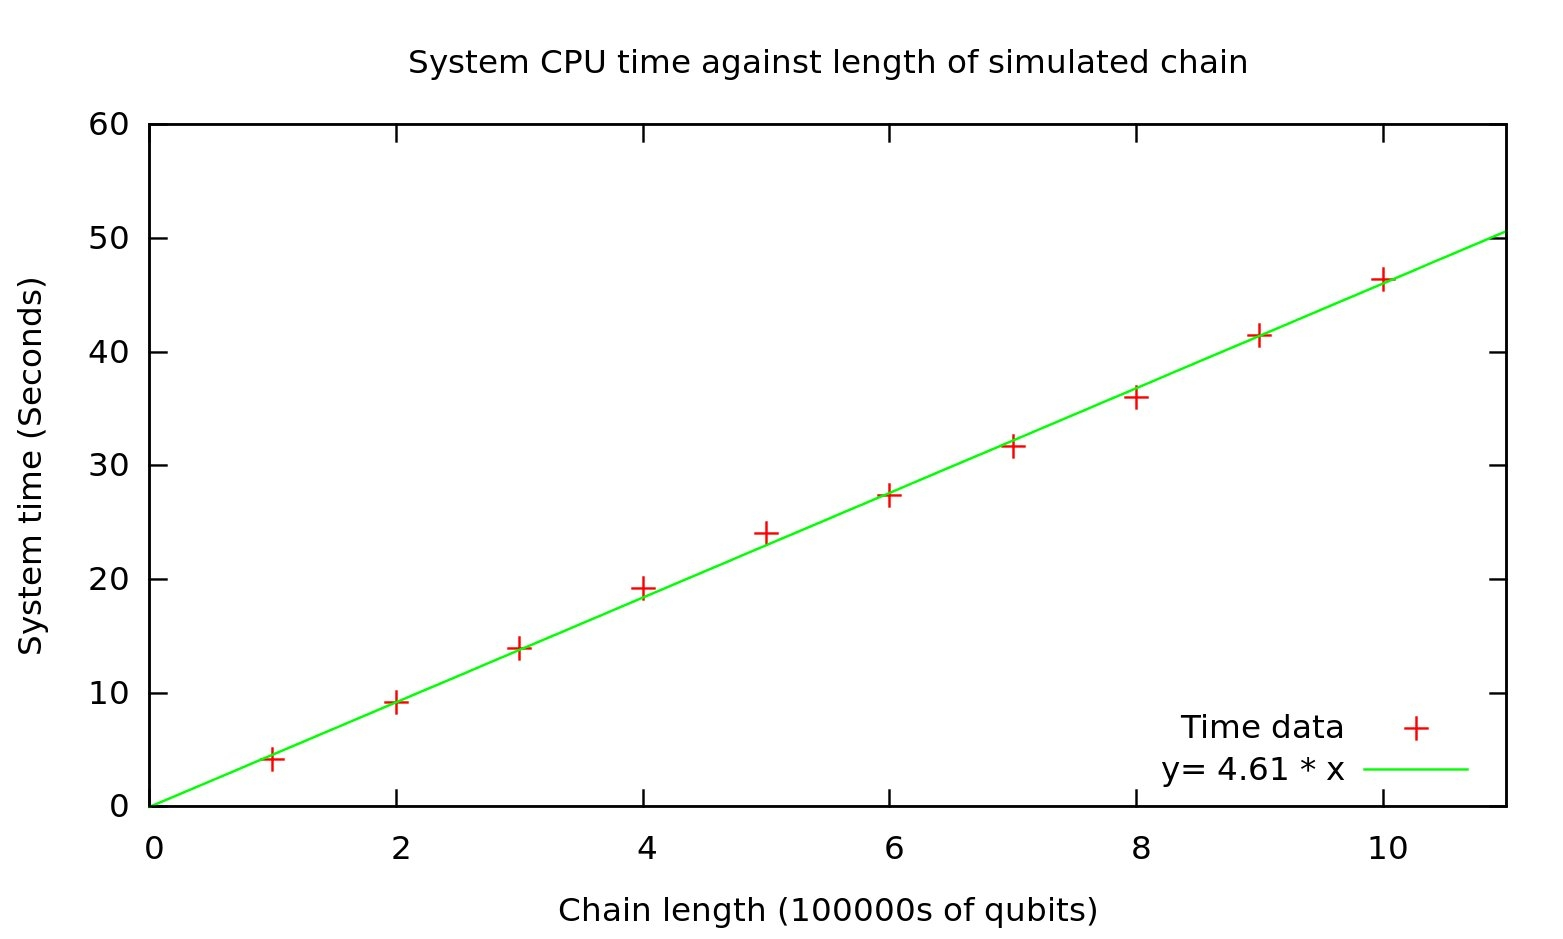
\includegraphics[scale=0.20]{gfx/singlechain_time_graph.jpg}
\caption{Graph of system CPU time against length of simulated chain for the SVD measurement method \label{fig:length_v_time_1}}
\end{figure}

In figure \ref{fig:length_v_time_1}, it can be seen that this relationship for the SVD method that removes qubits after each measurement has a linear relationship between time and chain length. This is as expected as the maximum matrix size is constantly low so the memory requirements for the program will be far lower than the projection operator method that require larger state vectors to be stored in memory. This result supports the claim made in \textit{"Cluster-state quantum computation"} \citep{nielsen_cluster-state_2006}, where it is shown that measurements on a quantum state can be efficiently simulated by a classical computer.


\begin{figure}
\centering
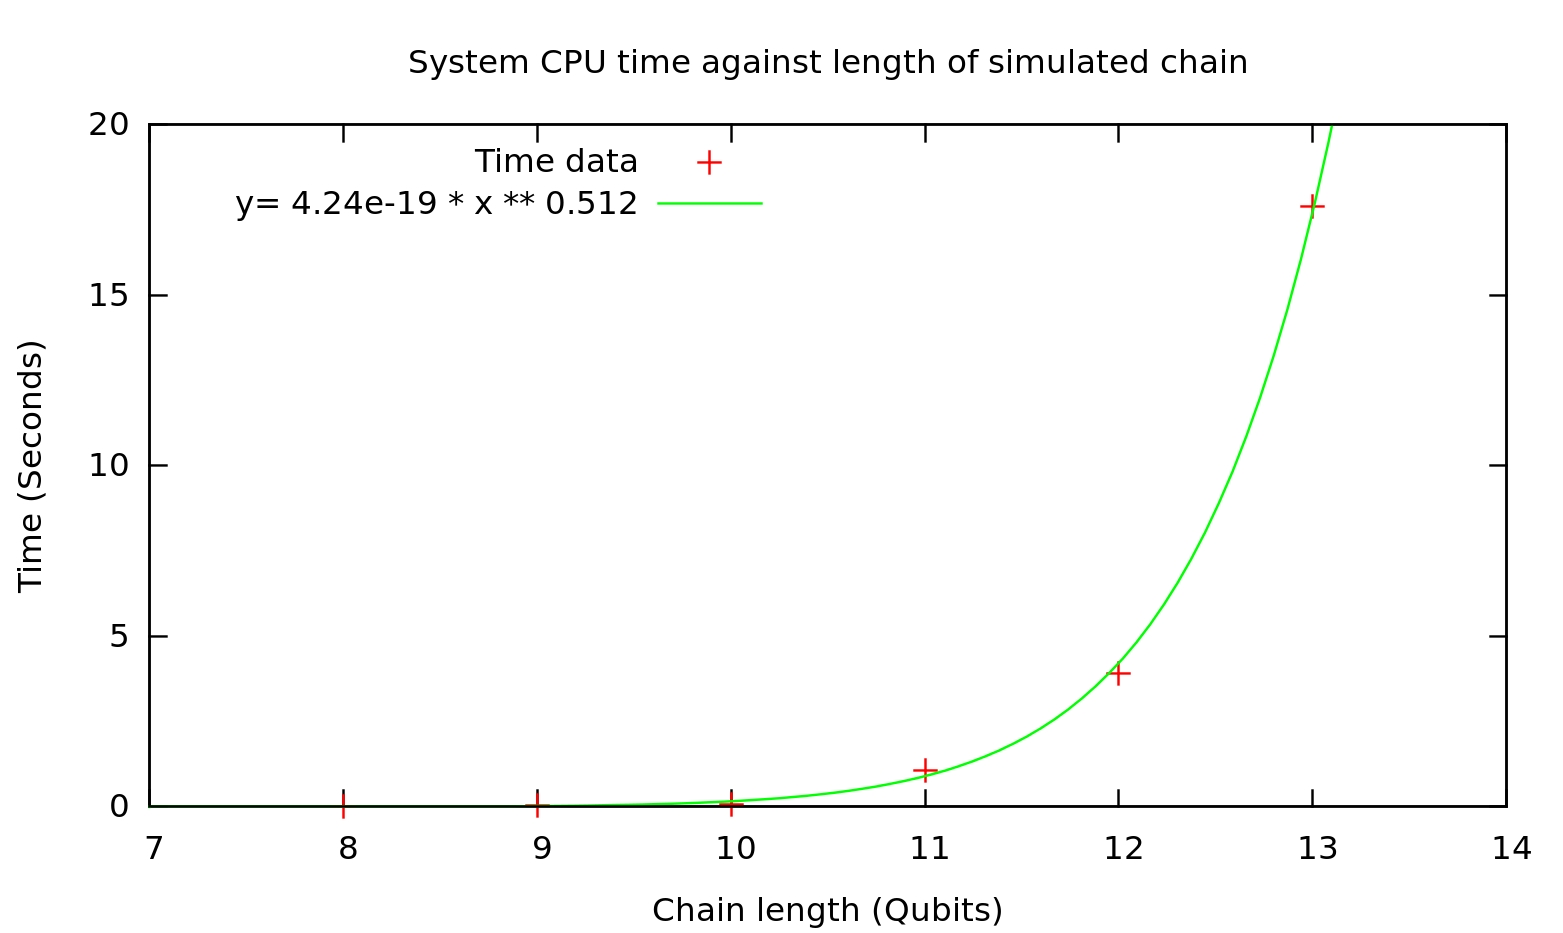
\includegraphics[scale=0.20]{gfx/timings2.jpg}
\caption{Graph of system CPU time against length of simulated chain for the projection operator measurement method \label{fig:length_v_time_2}}
\end{figure}

In figure \ref{fig:length_v_time_2} by contrast, it can be seen that the time scales approximately exponentially instead of the linear relationship from the previous figure. The parameters described in legend for the fitted curve are unlikely to be correct given the direction of the inflectional of the curve and are therefore best ignored. This implies a relationship of:

\begin{equation}
t \propto  \sim 2^{n}
\end{equation}


Which is as expected for the larger state vectors involved as the memory usage would need to scale in a similar manner which would explain the differences between the two simulations. This scaling is also indicative of the power of quantum computing because a real physical system would not have to scale in the same way allowing for efficient solutions to problems. When trying to simulate chains of larger than fourteen qubits in this manner the program seemed to time out before calculation, it is likely that this is because the program exceeded the memory limits of the machine so either more memory would be required to simulate larger systems or parts of the state vectors or operators would need to be stored on the hard disk, which would significantly bottleneck performance of the program.

The implications of this longer time extend onto future simulation of the error correction scheme which would require the same scaling factor when considering performance. Particularly as the simplest simulations of the error correction scheme would require at least six qubits to be simultaneously stored in memory along with their operators. However, as ten qubits can be fully simulated during the creation of cluster states and measurement in less than a second, simulations of the five qubit version of the error correction code would likely be able to be simulated easily for systems of two logical qubit. Unfortunately longer chains and multiple qubit gate operators would present a problem due to their significantly higher memory requirements given that they would likely require at least twenty five qubits which exceeds the current memory capacities of the machines used for simulation. In this case it would be necessary to use parallel processing to efficiently perform the simulation.


%----------------------------------------------------------------------------------------

\section{Conclusions}


While some progress was made in correcting problems with the program with measurements aside from the Pauli X measurement the goal of simulating the error correction scheme is still a long way from being achieved. The problem still seems to be present in the measurement itself given the in-correctness of the simulated Hadamard gate operation for all attempted methods of measurement simulation. It is therefore quite likely that there has been a fundamental misunderstanding of the theory behind the 'gate' operation itself which would need to be rectified for further progress to be made. Additionally there are clearly problems with the way by-product operators are calculated due to the mismatch between expected by-product and those used in the simulation and this will also have to be overcome or the operations required entered manually.

The investigations into the performance of the program did allow better insight into the kind of computational resources that would be required for simulation of the error correction scheme at least. It certainly seems that single logical qubit operations can be simulated with the same kind of hardware as used in this report while larger systems will require some orders of magnitude more. Hopefully this issue can be resolved for future versions of the program.
 % Chapter 8

%----------------------------------------------------------------------------------------
%	THESIS CONTENT - APPENDICES
%----------------------------------------------------------------------------------------

\appendix

%\part{Appendix} % New part of the thesis for the appendix

% Appendix A

\chapter{Appendix A: Code}
\label{app:code}

%----------------------------------------------------------------------------------------
\section{Single Chain Program}


\insertcode{"code_snippet/Code/clean/singlechain.F95"}{Single qubit gate program}

\section{CZ Operation Module}


\insertcode{"code_snippet/Code/clean/cz_op_module.F95"}{CZ Operation Module}

\section{Kronecker Product Module}


\insertcode{"code_snippet/Code/clean/kronecker_module.f95"}{Kronecker Product Module}

\section{Measurement Module}


\insertcode{"code_snippet/Code/clean/measurement_module.F95"}{Measurement Module}

\section{Fidelity Function}


\insertcode{"code_snippet/Code/clean/fidelity.F95"}{Fidelity Function} % Appendix A
% Appendix X

\chapter{Appendix B: Resources Used}
\label{app:resources}

The following contains details about computational resources used for the creation and running of the program.

%----------------------------------------------------------------------------------------


\section{Computer Used}

\begin{tabular}{l | r
}
\hline
Processor	     & Intel Core i7 2600K @ 3.40GHz \\
Memory	         & 8.00GB Dual-Channel DDR3 @ 802MHz                                   \\
Motherboard      & ASUSTeK Computer INC. P8P67 PRO \\
Disk Drive       & 931GB SAMSUNG HD103SJ  \\
Host Operating System  & Windows 8.1 Pro 64-bit \\
Guest Operating System & Linux Mint 13 Maya                     \\
\hline
\end{tabular}

\section{Compiler Settings}


The code was compiled using the gfortran compiler using flags -O3 -lblas and -llapack. -g was used for debugging. BLAS was used for matrix vector multiplication and inner product calculation.LAPACK was used for single value decomposition. % Appendix B - empty template
% Appendix A

\chapter{Appendix C: Additional Code}
\label{app:code}

%----------------------------------------------------------------------------------------
\section{Single Chain Program}
\insertcode{"code_snippet/Code/new_code/singlechain.F95"}{Single qubit gate program}

\clearpage
\section{Projection operators program}
\insertcode{"code_snippet/Code/new_code/fivechain.F95"}{Projection operators program}

\clearpage
\section{Kronecker Product Module}
\insertcode{"code_snippet/Code/new_code/kronecker_module.f95"}{Kronecker Product Module}

\clearpage
\section{Measurement Module}
\insertcode{"code_snippet/Code/new_code/new_measurement.F95"}{Measurement Module}

\clearpage
\section{Repeating single chain program}
\insertcode{"code_snippet/Code/new_code/singlechain_repeating.F95"}{Repeating single chain program}

\clearpage
\section{Repeating projection operators program}
\insertcode{"code_snippet/Code/new_code/fivechain_multi.F95"}{Repeating projection operators program} % Appendix A - Additional Code

%----------------------------------------------------------------------------------------
%	POST-CONTENT THESIS PAGES
%----------------------------------------------------------------------------------------

% Bibliography

\label{app:bibliography} % Reference the bibliography elsewhere with \autoref{app:bibliography}

\manualmark
\markboth{\spacedlowsmallcaps{\bibname}}{\spacedlowsmallcaps{\bibname}} 
\refstepcounter{dummy}

\addtocontents{toc}{\protect\vspace{\beforebibskip}} % Place the bibliography slightly below the rest of the document content in the table of contents
\addcontentsline{toc}{chapter}{\tocEntry{\bibname}}

\bibliographystyle{ieeetr}

\bibliography{Bibliography} % Bibliography

%% Colophon (a brief description of publication or production notes relevant to the edition)

\pagestyle{empty}

\hfill

\vfill

\pdfbookmark[0]{Colophon}{colophon}

\section*{Colophon}

This document was typeset using the typographical look-and-feel \texttt{classicthesis} developed by Andr\'e Miede. The style was inspired by Robert Bringhurst's seminal book on typography ``\emph{The Elements of Typographic Style}''. \texttt{classicthesis} is available for both \LaTeX\ and \mLyX: 

\begin{center}
\url{http://code.google.com/p/classicthesis/}
\end{center}

\noindent Happy users of \texttt{classicthesis} usually send a real postcard to the author, a collection of postcards received so far is featured here: 

\begin{center}
\url{http://postcards.miede.de/}
\end{center}
 
\bigskip

\noindent\finalVersionString % Colophon

%% Declaration

\refstepcounter{dummy}
\pdfbookmark[0]{Declaration}{declaration} % Bookmark name visible in a PDF viewer

\chapter*{Declaration} % Declaration section text

\thispagestyle{empty}

Put your declaration here.
\bigskip
 
\noindent\textit{\myLocation, \myTime}

\smallskip

\begin{flushright}
\begin{tabular}{m{5cm}}
\\ \hline
\centering\myName, \today \\
\end{tabular}
\end{flushright}
 % Declaration

%----------------------------------------------------------------------------------------

\end{document}
